\section{Bioetica 4: Etica della gestione e dell'organizzazione sanitaria}

\subsection{Introduzione del Dottor Muzzetto}

Oggi parleremo dell'etica della gestione dell'organizzazione sanitaria
con il Direttore Generale Fabi e il Direttore Sanitario Balestrino che
tratteranno un aspetto oggi forse poco noto a chi si avvicina alla
medicina. Anche nell'ambito della gestione ci sono degli aspetti
estremamente importanti che è giusto che chi fa il percorso della
Medicina conosca. Massimo Fabi è Direttore Generale della nostra Azienda
Ospedaliera Universitaria; ha fatto una carriera importante ed è uno dei
rappresentanti di rilievo nell'alveo delle direzioni generali italiane,
del coordinamento dei direttori generali. Il Dottor Balestrino ha
lavorato espressamente nell'ambito non solo delle direzioni sanitarie,
ma è stato anche Direttore Generale dell'Ausl di Pescara.

 \begin{figure}[!ht]
\centering
	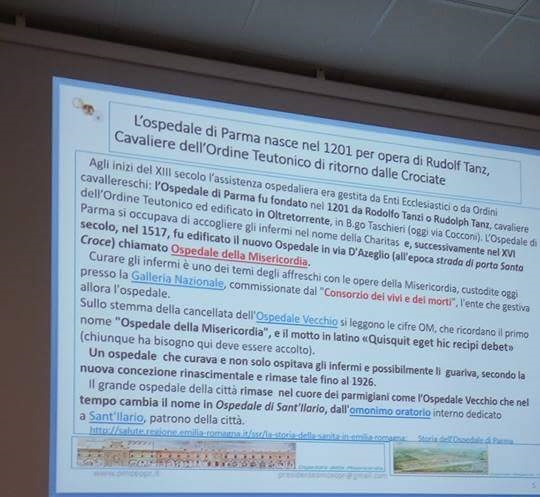
\includegraphics[width=0.8\textwidth]{32/image1.jpeg}
	\end{figure}

Oggi noi ci troviamo di fronte per parlare di una realtà che nacque nel
1201 come una struttura misericordiosa, una struttura per coloro che
avevano bisogno. Si fregiò di un titolo che ancora oggi rimane (e che è
riportato negli annali dell'ospedale): \emph{quisquit eget hic recepi
debet} (chiunque abbia bisogno deve essere accolto). Ancora oggi sulla
cancellata dell'Ospedale di Parma (in via D'Azeglio) c'è scritto questo,
perché era ed è uno dei segnali importanti della espressione di Parma
nell'ambito dell'assistenza e della cura. Da ospedale in mano ai
misericordiosi pian piano è passato al pubblico. Ciò da l'idea di come
il privato, e non soltanto la Chiesa, potesse dare una mano a chi aveva
bisogno. Da qui fino all'ospedale del 1500 che poi è cambiato diventando
un ospedale molto avanzato. L'Ospedale di Parma è stato uno dei primi a
mettere i bambini da una parte e gli adulti dall'altra, perché un tempo
negli ospedali i bimbi e gli adulti, con patologie estremamente diverse,
venivano messi insieme. Già questa sensibilità di spostarli e di curarli
diversamente da l'idea di come fosse avanzato il modo di vedere la
salute e la sanità da parte anche dei parmigiani, quindi è nota di
grande merito.

 \begin{figure}[!ht]
\centering
	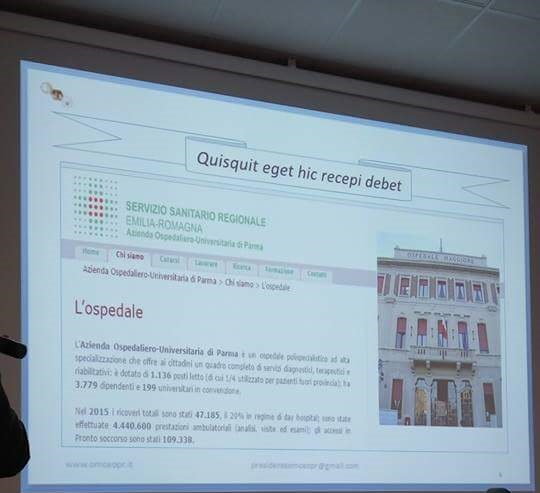
\includegraphics[width=0.8\textwidth]{32/image2.jpeg}
	\end{figure}

Oggi l'ospedale è la prima azienda di questa provincia, sia per
complessità sia per numero di persone che vi lavorano. Passo ora la
parola al Dottor Balestrino che ci parlerà appunto di etica della
gestione della sanità pubblica.

\subsection{Introduzione del Direttore sanitario Balestrino}

Siamo in una dimensione concettuale che è inflazionata dal concetto di
etica e da tutto ciò che è correlabile direttamente o indirettamente
all'agire etico e di conseguenza a volte si corre il rischio di cadere
nello scontato o nel banale (lo diventa un po' meno quando ci si trova
dietro ad una scrivania o a prendere delle decisioni). La visione etica
della situazione, e anche delle possibili prospettive che nascono da
quella decisione, non può prescindere dalle altre considerazioni che
normalmente costituiscono il vivere quotidiano di chi fa gestione
(chiamiamolo con un termine più adeguato, \emph{managerialità}). L'etica
non è appannaggio di chi prende decisioni perché l'etica è anche una
costante di chi giornalmente vive una dimensione lavorativa a tutti i
gradi e a tutti i livelli, perché ogni giorno ci troviamo in molteplici
situazioni che comportano delle scelte decisionali in cui la valenza
etica ha un suo carattere, a volte molto spesso predominante,
soprattutto all'interno delle organizzazioni.

In questa presentazione vorremmo trattare questi argomenti:

\begin{itemize}
\item[1.]
  \emph{Inquadramento dell'etica secondo la visione di chi fa
  organizzazione}. Il tema dell'etica in ospedale sarà un momento
  importante di questo nostro incontro, ma non può prescindere da che
  cosa vuol dire una visione etica delle azioni in ospedale all'interno
  di una rete più complessiva di integrazione di sanità ospedaliera con
  sanità territoriale.
\item[2.]
  \emph{Etica in termini di responsabilità, di cultura della
  trasparenza}
\item[3.]
  \emph{Esempi pratici} di decisioni di grande portata, supportate da
  argomenti di carattere etico.
\end{itemize}

\subsection{Cosa è l'etica e di cosa si occupa}

 \begin{figure}[!ht]
\centering
	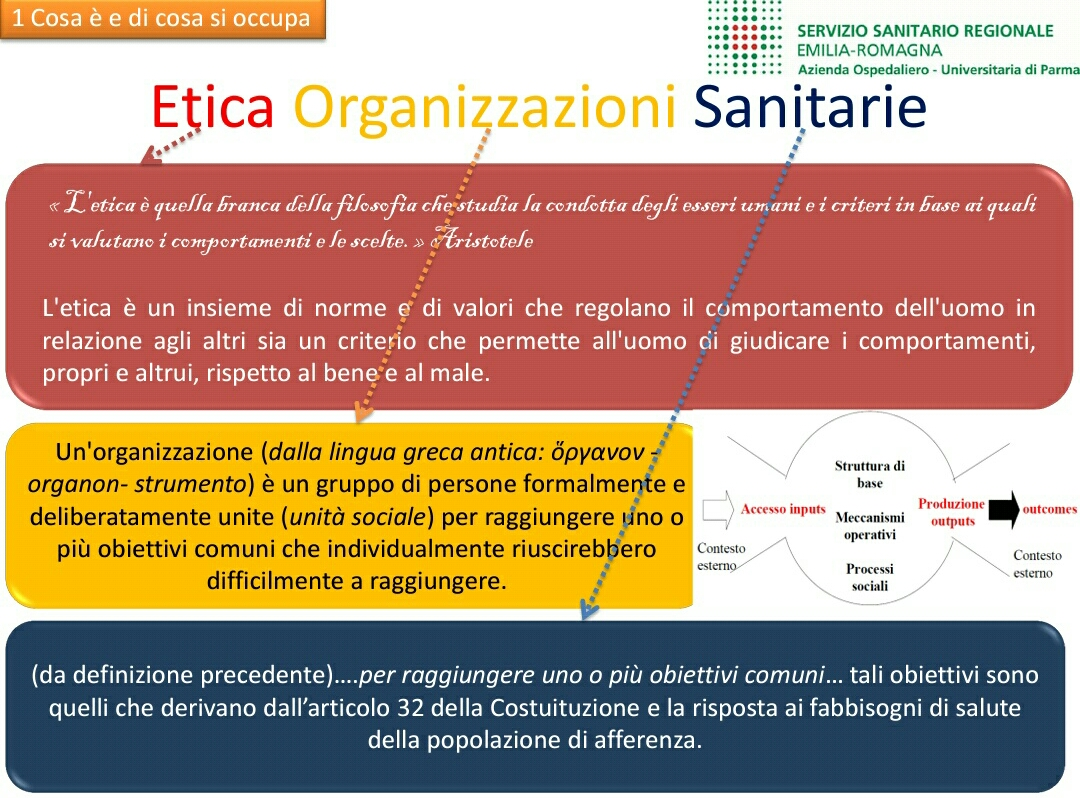
\includegraphics[width=0.8\textwidth]{32/image3.jpeg}
	\end{figure}

Coniughiamo tre termini: Etica, Organizzazione, Sanità.

L'\textbf{etica} è un insieme di norme e di valori che regolano il
comportamento dell'uomo in relazione agli altri quindi è un concetto
sovrano che attiene alla sfera comportamentale e alla sfera delle
relazioni degli uni e degli altri.

\textbf{Organizzazione}: è il concetto chiave che associamo al primo.
Anche voi dovete incominciare a meglio inquadrare che cosa voglia dire
essere parte di una organizzazione e che cosa voglia dire essere una
organizzazione. Essere una organizzazione vuol dire appartenere ad un
gruppo di persone che sono formalmente e deliberatamente unite perché
costituiscono un gruppo sociale, una unità sociale, finalizzata al
raggiungimento di uno o più obiettivi comuni che individualmente
difficilmente riuscirebbero a raggiungere. Il concetto
dell'organizzazione che predomina in questa visione è un accesso di
input, di risorse, di fattori produttivi e una uscita di output e di
outcome (output=quantitativi mentre outcome=esiti in termini di salute)
che caratterizzano più appropriatamente una organizzazione come quella
sanitaria che di fatto è una organizzazione destinata a produrre salute.
All'interno di questa organizzazione funziona una serie complessa,
eterogenea e varia di meccanismi sociali, relazionali, comportamentali
(e supportati chiaramente dall'impiego appropriato e nel giusto momento
di risorse) tali che quell'innesco di input si trasformi poi in output e
in outcome, con al centro ovviamente la persona come beneficiario
primario del lavoro dell'organizzazione. Ecco perché noi stiamo parlando
dell'etica dell'organizzazione sanitaria che ha come obiettivo la
salute, secondo l'articolo 32 della Costituzione; solamente chi è
all'interno dell'organizzazione riesce a ben comprendere la valenza, lo
spessore e l'importanza etica di dover presidiare, difendere e sostenere
giornalmente il significato di quell'articolo in termini di riposta ai
fabbisogni di salute della popolazione.

\subsubsection{Ambiti di applicazione dell'etica organizzativa}

 \begin{figure}[!ht]
\centering
	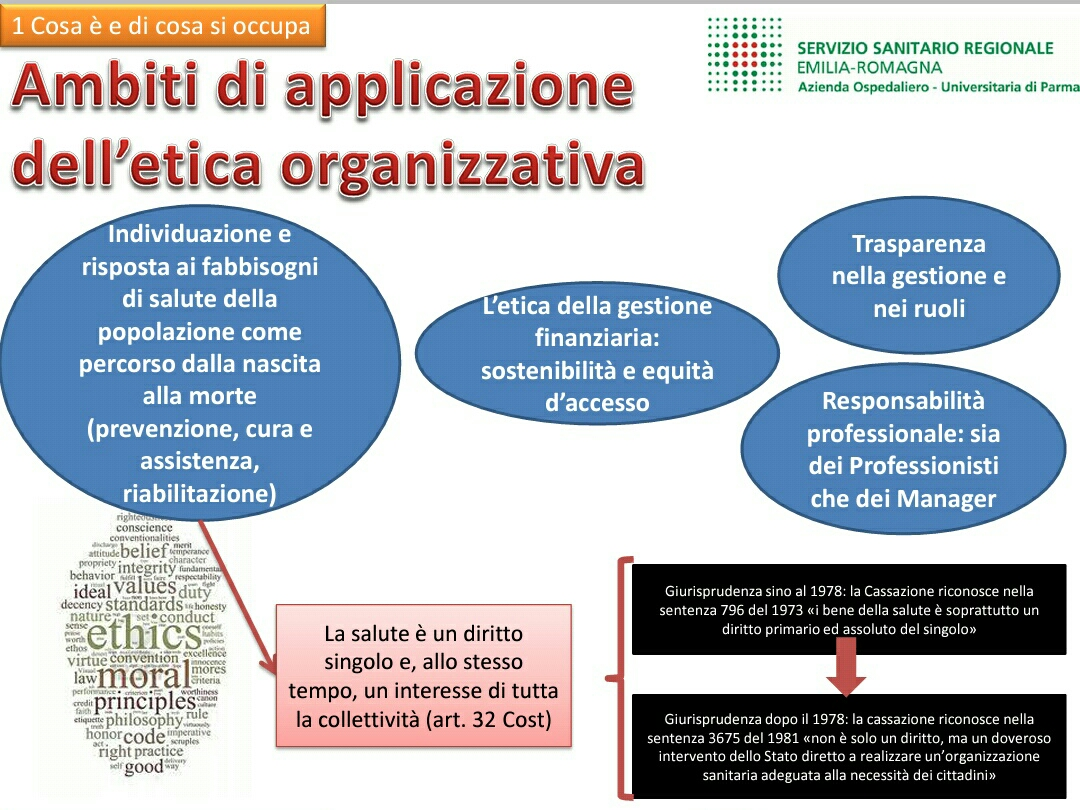
\includegraphics[width=0.8\textwidth]{32/image4.jpeg}
	\end{figure}

Se non facciamo a monte un'analisi dei \emph{bisogni di salute della
popolazione} (come percorsi, quindi dalla prevenzione, alla cura,
all'assistenza, alla riabilitazione) non abbiamo il peso del lavoro che
ci aspetta e di come quel lavoro vada orientato e di come dobbiamo
fissare degli obiettivi a monte del lavoro e delle scelte che facciamo.
Esiste un'\emph{etica della gestione finanziaria}, anche questa è
un'etica! Un gestore (un direttore di struttura, un direttore generale,
un direttore sanitario, un direttore di Struttura Complessa, un medico,
un coordinatore) si trova a dover giornalmente pesare le risorse di cui
dispone in relazione ai bisogni e in relazione anche all'appropriatezza
dell'utilizzo di quelle risorse. E poi esiste \emph{un'etica nella
trasparenza nella gestione e nei ruoli} e un'\emph{etica che riguarda la
responsabilità professionale,} sia dei Manager che dei professionisti.

Su tutto ciò si scrive il concetto di salute come diritto del singolo e
nel contempo interesse della collettività, perché quando agiamo sul
singolo ci dobbiamo sempre chiedere quali sono gli effetti di quel
problema di salute rispetto alla comunità di riferimento cui quel
singolo potrebbe aver recato o meno un nocumento, secondo una visione
che nel corso di questi anni ha cambiato alcuni paradigmi di lettura.
L'articolo 32 della Costituzione parla del bene salute come diritto
primario e assoluto del singolo (che confermiamo nel suo valore e nel
suo spessore). Poi c'è stato l'avvento delle normative di settore che
hanno innovato, ogni 20-25 anni circa, la sanità (la 833 del `78, la 502
del `92, per giungere poi ai giorni nostri e ai piani di riordino anche
degli standard ospedalieri). Tutto ciò ha cambiato un attimo la modalità
di leggere il concetto di salute: essa è sì un diritto del singolo, ma
diventa anche un doveroso intervento dello Stato diretto a realizzare
un'organizzazione sanitaria adeguata alle necessità dei cittadini. È
cambiato il senso etico della prospettiva. Il diritto esigibile rimane
tale e dinanzi ad esso il medico è ossequioso (ed è la persona, il
professionista più altamente responsabilizzato in quel dualismo di
rapporto specifico che connota il contratto tra medico e paziente); su
questo si innesta poi l'appartenenza di quel soggetto professionale ad
una comunità (che è l'organizzazione sanitaria che lo esprime) la quale
di per sé è responsabile a monte di quel diritto esigibile del singolo
che appartiene alla comunità e quindi della comunità tutta. Cambia un
filo conduttore di logica che investe i gestori, investe i singoli nel
momento in cui sono espressioni di un sistema organizzativo cui essi
appartengono. Questo è un cambio paradigmatico di modo di pensare e
anche di esercitare le proprie responsabilità.

 \begin{figure}[!ht]
\centering
	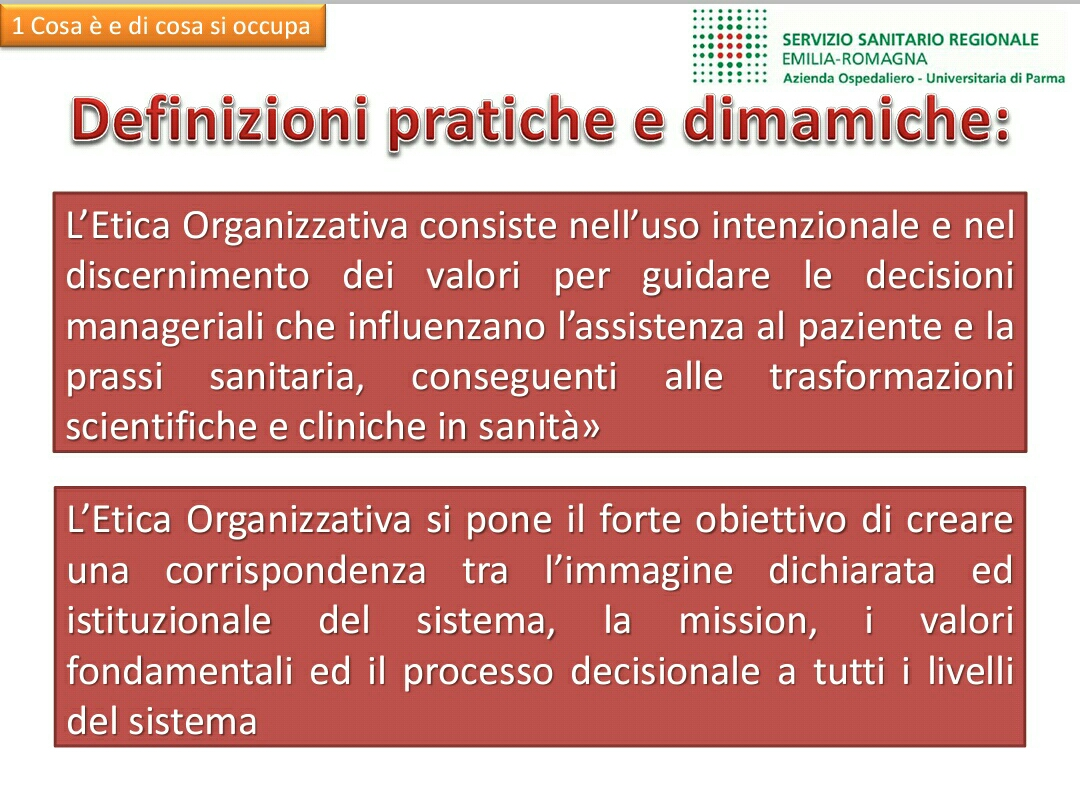
\includegraphics[width=0.8\textwidth]{32/image5.jpeg}
	\end{figure}

L'etica organizzativa consiste nell'uso intenzionale e nel discernimento
dei valori per guidare le decisioni manageriali che influenzano
l'assistenza al paziente e la prassi sanitaria, conseguenti alle
trasformazioni scientifiche e cliniche; non esiste un'etica statica,
esiste un'etica che si trova giornalmente a dover fare i conti con il
progresso. Meno male, siam contenti, però nel momento in cui abbiamo una
trasformazione scientifica e clinica ci sono delle domande che il
gestore si deve porre anche dal punto di vista etico: ``la doto o meno
la mia struttura organizzativa dell'ultimo modello di ecografo? Rispetto
a che target di popolazione? Di tutti quelli che passano? Uno specifico?
Come incomincio, come faccio, con quali risorse? Utilizzo o meno quel
determinato farmaco di ultima generazione? Ma si deve sempre utilizzare
il farmaco di ultima generazione?'' Ecco, sono temi rispetto ai quali
non è solamente la scelta clinica a fare da padrone, nella quale cioè il
professionista è solo con se stesso all'interno della sua cerchia
professionale di riferimento. È una scelta di un sistema organizzativo,
è l'etica dell'organizzazione. L'etica organizzativa si pone il forte
obiettivo di creare una corrispondenza tra l'immagine dichiarata ed
istituzionale del tema, la sua \emph{mission}, i suoi valori
fondamentali e il processo decisionale a tutti i livelli. Non possiamo
pensare che un'organizzazione sanitaria in quanto tale e per tale
invocata dal soggetto fruitore, cittadino o collettività, non
corrisponda a degli standard di base per rispondere ai bisogni di quella
collettività. Significa che a monte se un sistema organizzativo vuol
essere etico deve fare un'operazione di dichiarata trasparenza, nel
senso che deve dichiarare qual è la propria \emph{mission}, la propria
faccia al pubblico, quelli che sono i propri valori fondamentali, ma
quali sono anche i livelli su cui si articola il proprio sistema di
valori. Quando leggete (basta aprire internet e andare a cliccare su
qualsiasi azienda sanitaria o ospedale o sistema che si voglia) la
declinazione della \emph{mission} del sistema dei valori e dei livelli
di realizzazione di quei valori non è un atto pubblicitario, e guai se
chi articola quel tipo di espressione di visibilità lo facesse calcando
delle tinte e creando delle illusorie aspettative, che poi il sistema
nella sua realtà non concretizza. Questa è etica organizzativa, che
significa quindi aver ben chiaro (da parte di chi si espone ma anche di
chi agisce e decide) qual è la \emph{mission} del sistema che governa,
quali sono i punti di forza compresi quelli valoriali e quali sono i
livelli decisionali all'interno dei quali e con i quali ci si può
muovere per realizzare la missione del sistema. Quindi vi ho già
anticipato che cosa vuol dire un'organizzazione che rispetta la propria
\emph{mission}; io vi ho molto sinteticamente elencato quelli che sono
gli elementi etici fondanti un'organizzazione. Non troverete sistema
organizzativo che non abbia una scansione di questi valori etici
rispetto ai quali si trova giornalmente a doversi confrontare nel
momento in cui esercita delle scelte.

 \begin{figure}[!ht]
\centering
	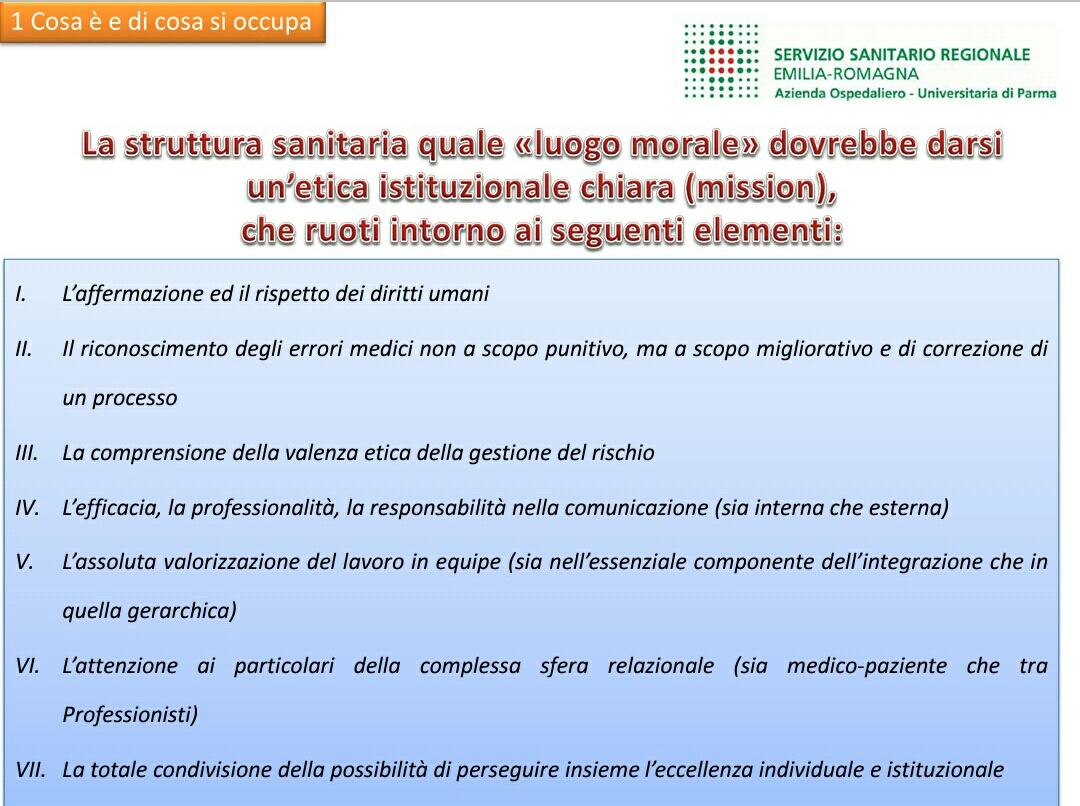
\includegraphics[width=0.8\textwidth]{32/image6.jpeg}
	\end{figure}

Partiamo dal concetto del diritto umano (già declinato in termini di
individualità e collettività) poi andiamo anche all'interno di
caratteristiche proprie dell'organizzazione (che sono quelle che più
marcatamente incidono e con le quali ci si confronta giornalmente per la
realizzazione dei valori etici): il lavoro di equipe, l'attenzione alla
sfera relazionale tra medico e paziente e anche tra professionisti, e
soprattutto il senso della condivisione della possibilità di perseguire
l'eccellenza individuale ed istituzionale. Quando si dirige o si
appartiene ad una struttura aziendale che si prefigura come centro HUB
di riferimento e come centro di eccellenza (in quanto centro di
riferimento per determinate patologie o trattamento di patologie o
comunque percorsi) è necessario che il concetto di eccellenza vada
declinato con la giusta misura. Se ci si mette una coccarda, quella
coccarda ce la si può mettere però a quel punto la si rispetta in tutte
le sue componenti, compreso il senso di sacrificio per tenere quella
coccarda: 365 giorni all'anno, senza festività, la notte, il giorno, in
qualsiasi condizione, con qualsiasi tempo climatico, esterno ed interno
all'organizzazione, andando a promuovere soprattutto quella che è la
condivisione nel tenere in piedi quell'eccellenza. Il sapere
professionale, che io non chiamo più sapere ma competenza (perché la
competenza è un insieme di valori, tra cui il sapere) è il frutto di un
lavoro quotidiano, costante, giornaliero che permea il singolo e la
collettività di appartenenza, perché esso lo ha sostenuto in relazione
agli sforzi e ai sacrifici che servono per gestire quella competenza.
Questo è importante per chi fa il mio mestiere, e lampante rispetto
all'interlocutore cui mi trovo di fronte. Vi posso assicurare che mi
basta mezza frazione di secondo per sapere quando l'interlocutore vuole
ingannare la gestione, ma alla fine inganna solo se stesso, tanto peggio
inganna il cittadino. Quello diventa il patto che può nascere, ma che
potrebbe in qualche maniera non spezzarsi ma sicuramente incrinarsi, in
un giudizio valutativo che costituisce una componente essenziale della
dimensione dell'equilibrio dell'etica organizzativa.

 \begin{figure}[!ht]
\centering
	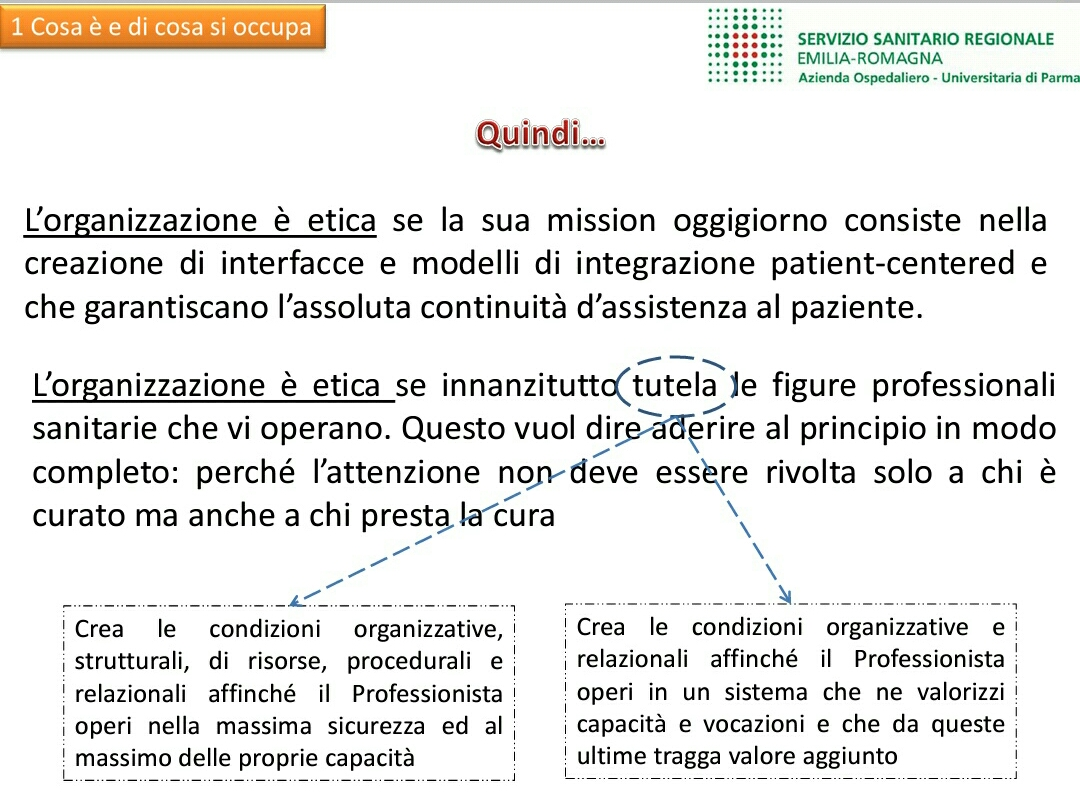
\includegraphics[width=0.8\textwidth]{32/image7.jpeg}
	\end{figure}

Quindi l'organizzazione è etica se la sua \emph{mission} oggigiorno
consiste nella creazione di interfacce e modelli di integrazione
centrati sul paziente che garantiscano la continuità dell'assistenza.
Non siamo più in un sistema organizzativo in cui il paziente entra in
ospedale, gli curiamo il sintomo e molto spesso anche la patologia e lo
rimandiamo fuori. Non funziona più così, si agisce a monte, nel momento
in cui il paziente entra all'interno di un target di rischio; si ragiona
anche a valle nel momento in cui quel paziente, che ha superato la sua
acuzie per cui l'ospedale esiste, ritorna nel proprio nucleo sociale di
cui la medicina territoriale è un punto di forza, è un punto di
rappresentatività, è un punto di riferimento delle sue componenti.
Allora siamo troppo soliti pensare al nostro medico di medicina
generale, però egli è a sua volta un pezzo di un sistema organizzativo
che noi chiamiamo assistenza sanitaria territoriale primaria. Quello che
si sta sempre più evidenziando non è più la singolarità della relazione
del paziente con il professionista, ma del paziente con dei sistemi
organizzativi che hanno dei supporti etici e deontologici in base ai
quali agiscono. L'organizzazione etica innanzitutto tutela le figure
professionali che vi operano, questo vuol dire aderire al principio in
modo completo; l'attenzione non deve essere solo verso chi è curato, ma
anche verso chi cura. Attenzione perché nel momento in cui si fa un
esercizio etico non si fa una difesa ad oltranza. La relazione
all'interno di un sistema organizzativo non è una relazione che può
essere rigida ma non può nemmeno essere una relazione paternalistica, se
sistema etico deve essere. È una relazione nella quale anche nello
scambio tra pari ci si scambiano delle vedute, si fanno delle
affermazioni fondate su regole di principio, oltre che su regole
tecnico-professionali ovviamente; esse costituiscono il driver del modo
di ragionare sul caso specifico, sull'evento, sulle situazioni che sono
oggetto di riflessione. Il concetto di tutela ha, in termini di etica
organizzativa, oggi una doppia lettura: tutela vuol dire agire, creare
delle condizioni organizzative tali da garantire all'operatore
sicurezza, espressione delle proprie capacità professionali, ma
significa anche creare delle condizioni organizzative e relazionali
affinché il professionista operi in un sistema che ne valorizzi le
capacità e le vocazioni. Un professionista non può prescindere dalla
capacità di appartenere ad un sistema che lo sostiene quando merita di
essere sostenuto e lo promuove quando è il momento di essere promosso
(quando questo professionista ha raggiunto dei livelli di competenza
professionale, umana, di globalità del sapere e del saper essere, e
quindi del saper fare).

\subsection{Focus sull'ospedale}

 \begin{figure}[!ht]
\centering
	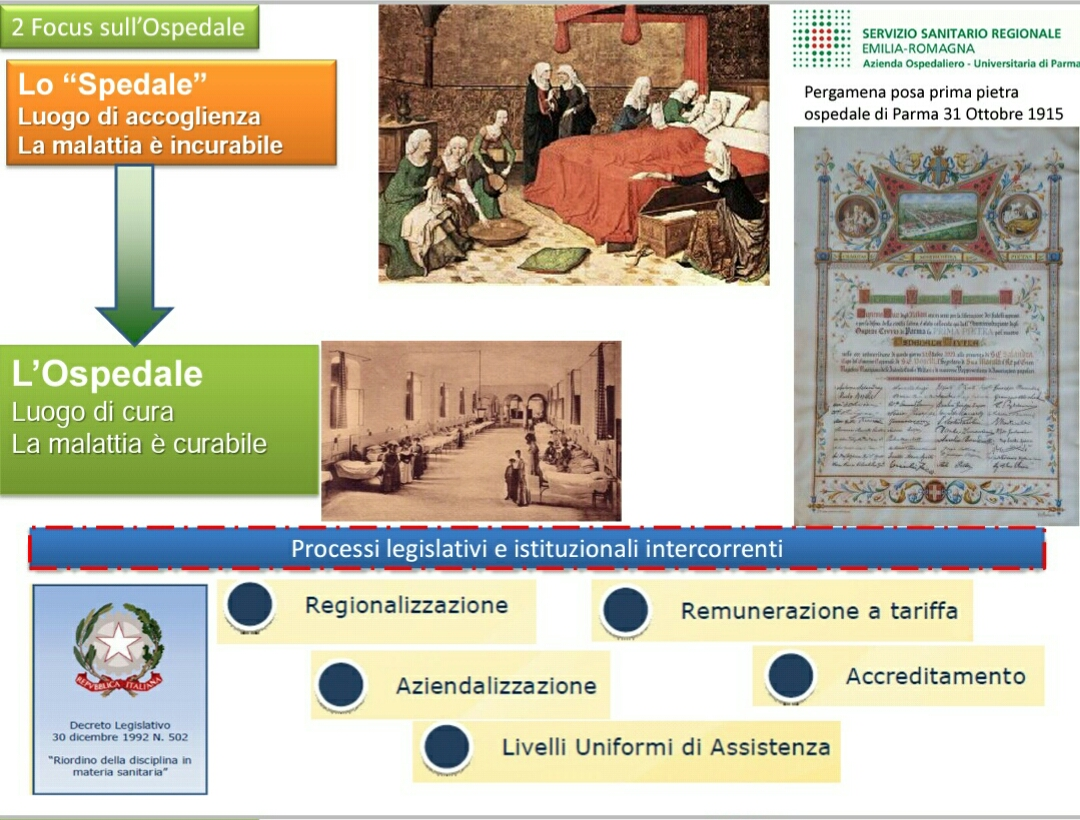
\includegraphics[width=0.8\textwidth]{32/image8.jpeg}
	\end{figure}

Lo diceva il nostro presidente dell'Ordine: siamo passati da ospedali
come luoghi di accoglienza (luoghi di malattie che molto spesso erano
incurabili) ad ospedali come luoghi di cura (dove la malattia è
curabile) e a sistemi organizzativi per cui la malattia è prevenibile.
Si è passati attraverso una serie di mutamenti che hanno caratterizzato
la sanità se non altro dal `78 in poi: i processi di regionalizzazione,
i processi di aziendalizzazione, i livelli uniformi di assistenza,
l'accreditamento.. ognuno di essi rappresenta una maniera per trasferire
o per creare delle condizioni standardizzate di offerta di servizi e di
proposta di prestazioni (non solamente quindi un'offerta gelida di
servizi ma una proposta articolata di un sistema organizzativo che si sa
esprimere nelle proprie capacità prestazionali da poter realizzare i
propri obiettivi istituzionali e la propria \emph{mission}).

 \begin{figure}[!ht]
\centering
	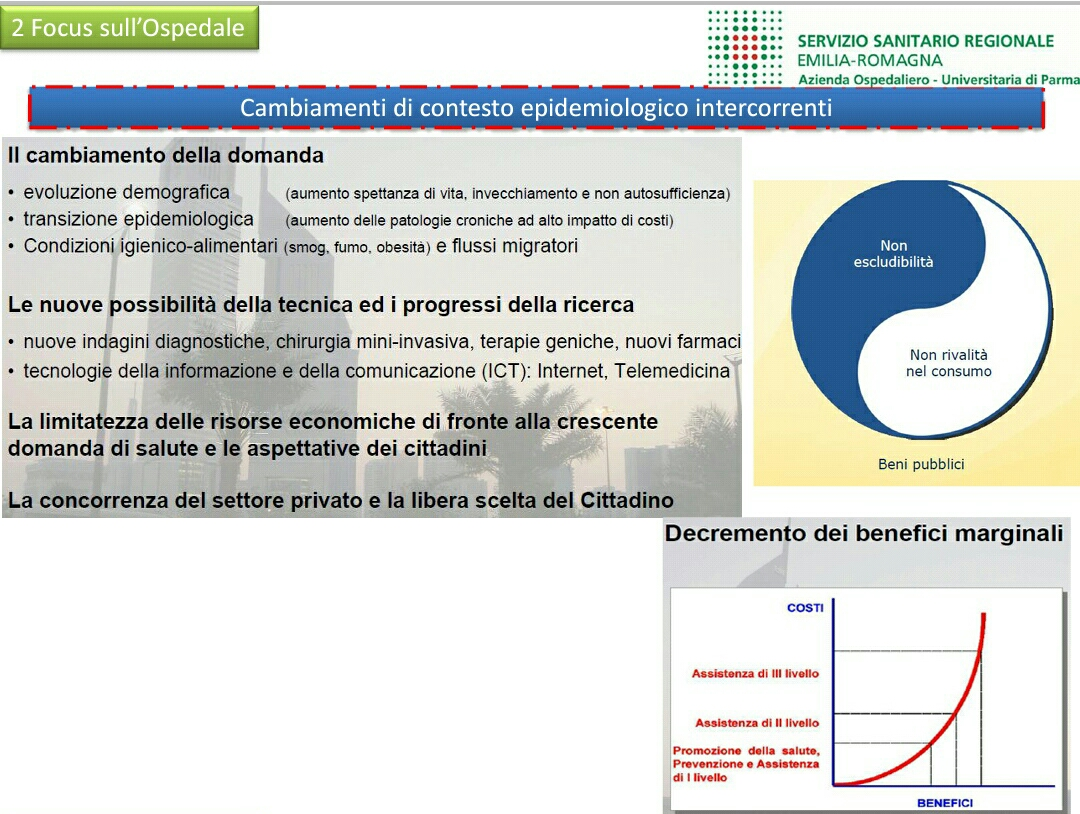
\includegraphics[width=0.8\textwidth]{32/image9.jpeg}
	\end{figure}

Sono successe tante cose ... C'è stato un cambiamento della domanda,
frutto dell'evoluzione demografica, della transizione epidemiologica,
dei flussi migratori, delle condizioni igienico-alimentari di una
popolazione che è passata attraverso varie epoche e oggi ne vive
anch'essa una. Ci sono stati progressi nella ricerca, nella tecnica;
sono cambiate le relazioni socioeconomiche tra i target di popolazione
ed è cambiato anche il lavoro. Non è appropriato parlare di concorrenza
e nemmeno di competizione, ma di \emph{presenza di un soggetto privato
accreditato}, paritariamente attestantesi come sistema dei valori in
relazione con il pubblico; esso quindi deve esercitare un proprio ruolo,
purchè sia un ruolo coerente con la propria \emph{mission}, e viene
accettato da un contesto pubblico affinchè faccia quel tipo di attività.
Non è detto che noi andiamo dal privato per fare il grande intervento di
trapianto. È meglio un privato che sappia fare degli interventi buoni,
ottimi, appropriati di appendicectomie, di ernie, di varici perché così
consente alla popolazione di risolvere un bisogno che essa ha e che non
mancherà; inoltre serve anche a delimitare la sfera d'azione di chi fa
un lavoro di maggiore spessore per competenza, caratteristiche
organizzative e tecnico-professionali, che è colui che deve fare i
trapianti, lo mette in condizione di equilibrio, è un sistema che è
eticamente e organizzativamente in equilibrio.

Chi fa organizzazione deve sempre avere il concetto etico della gestione
delle risorse: più alziamo i livelli di complessità più la curva si
impenna in termini di costi; chiaramente siamo impegnati a dover gestire
non solo le risorse che abbiamo ma anche l'equilibrio di quelle risorse
rispetto a una domanda, il che significa che deve sempre arrivare una
domanda che sia appropriata; promozione della salute, prevenzione e
assistenza di primo livello ci consentono di far fronte a quella domanda
che non è ancora tale da essere secondo e terzo livello. È una
mediazione costante, ma è un vivere eticamente anche scelte che servono
a gestire il sistema nel suo complesso.

Quando parliamo di aziende ospedaliere, di presidi ospedalieri, stiamo
parlando di ambiti organizzativi ad alta tecnologia: luoghi appropriati
per assistenza appropriata. I team, la progettazione partecipata, ma
anche la flessibilità strutturale sono elementi fondamentali. Un
ospedale deve essere solido (pareti in cemento armato) e flessibile, non
rigido. Avere l'ospedale flessibile vuol dire costruire anche
architettonicamente un ospedale in grado di modificarsi nel tempo e di
adeguarsi ai bisogni. La flessibilità strutturale è innanzitutto frutto
della nostra flessibilità ideale, perché se siamo rigidi nella
progettazione non saremo in grado di adattarci al divenire dei tempi.
Dobbiamo essere flessibili sin dal momento della progettazione, a volte
anche ritornando sulle nostre decisioni, ma avendo ben chiari gli
elementi valoriali ed etici. È troppo facile pensare a una scelta quando
le vie dinanzi sono due..molto spesso la scelta si fa e diventa scelta
(in cui il sistema dei valori ha la sua dominanza) quando le vie davanti
incominciano a essere 5, 6, 7, 10.. allora interviene un sistema di
pesatura. È troppo facile scegliere quando i margini di una via sono
all'80\%, (e quindi al 20\% di marginalità negativa) e l'altra via è
all'opposto in termini di marginalità positive o negative. Non è più una
scelta, diventa un obbligo. Questo è il tema che porta avanti
quotidianamente chi fa gestione, ma anche chi giornalmente si trova a
dover ragionare rispetto a un paziente che ha una condizione di salute,
che ha una condizione socio-sanitaria, che ha una condizione di
prospettiva di vita, che ha una condizione di prospettiva ambientale,
economico, familiare.. Arriva tutto, perché arriva l'essere umano
nell'organizzazione sanitaria. E non possiamo limitarci ad essere dei
tecnici. Oggi il medico è un professionista che dovrà sempre più
compendiare nel quadro delle proprie competenze il proprio sapere
tecnico-professionale col proprio sapere relazionale e organizzativo e
anche con la propria capacità di vivere la propria etica come uomo e
come professionista.

 \begin{figure}[!ht]
\centering
	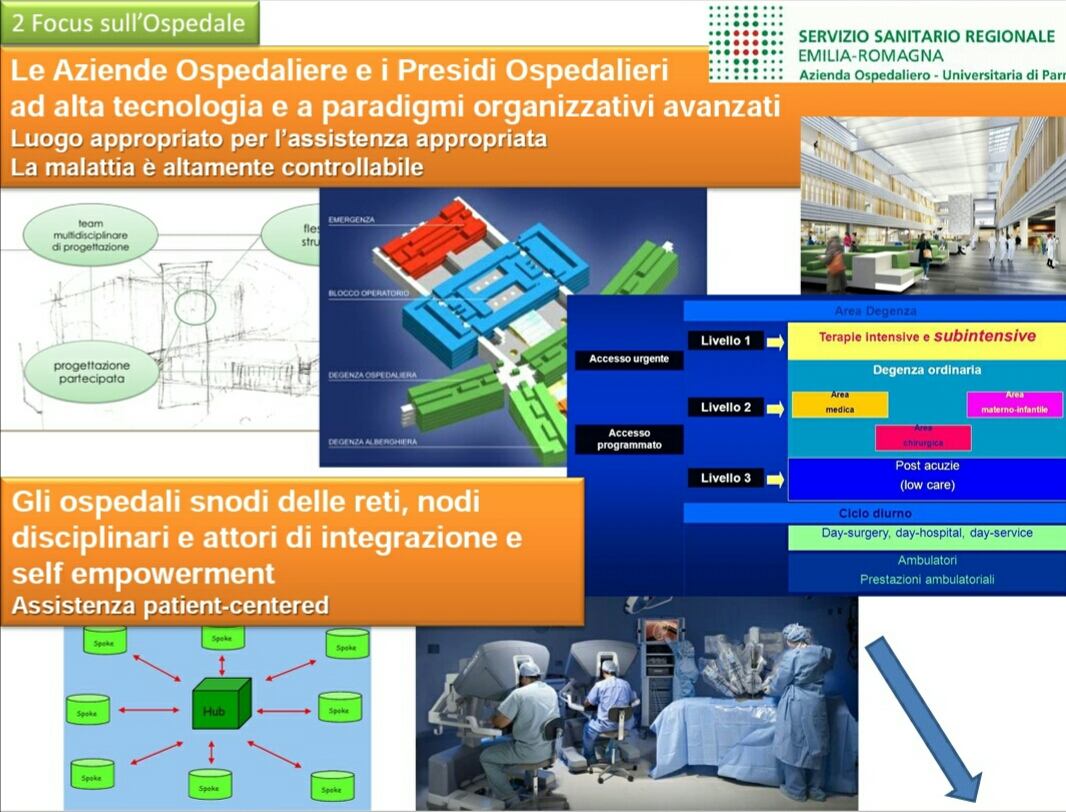
\includegraphics[width=0.8\textwidth]{32/image10.jpeg}
	\end{figure}

Questa è l'articolazione di un ospedale nella concezione classica di chi
fa ospedale: l'emergenza, i blocchi operatori, le degenze ospedaliere.
Soffermiamoci sul concetto di degenza alberghiera. Io molto spesso mi
trovo a dover discernere: preferisco una condizione alberghiera in quel
momento migliore oppure la sicurezza delle cure e del risultato se vado
in ospedale per curarmi? E se porto un mio caro in ospedale? Sono scelte
all'ordine del giorno. È una scelta del paziente che va orientato e del
gruppo familiare, molto spesso rischianti in proprio perché non è detto
che anche la persona più altolocata si renda conto del rischio di
scegliere un ambiente che non abbia delle caratteristiche di sicurezza
rispetto ad altri. Anche il soggetto istituzionale magari pretenderebbe
di alzare il livello alberghiero, ma esso deve garantire innanzitutto un
risultato in termini di outcome, che rimane uno dei prioritari obiettivi
di un direttore sanitario nel momento in cui legge l'evoluzione della
situazione di una persona o di un target di popolazione rispetto a dei
fenomeni di patologia. Sono scelte, sono tra l'altro scelte legittime,
sono ambiti di scelta. Ogni giorno ci si troverà a dover scegliere
perché il tema dell'etica è sempre lo stesso: che scelta faccio rispetto
alla mia sfera di comportamenti o a quella del sistema a cui appartengo
o che dirigo.

 \begin{figure}[!ht]
\centering
	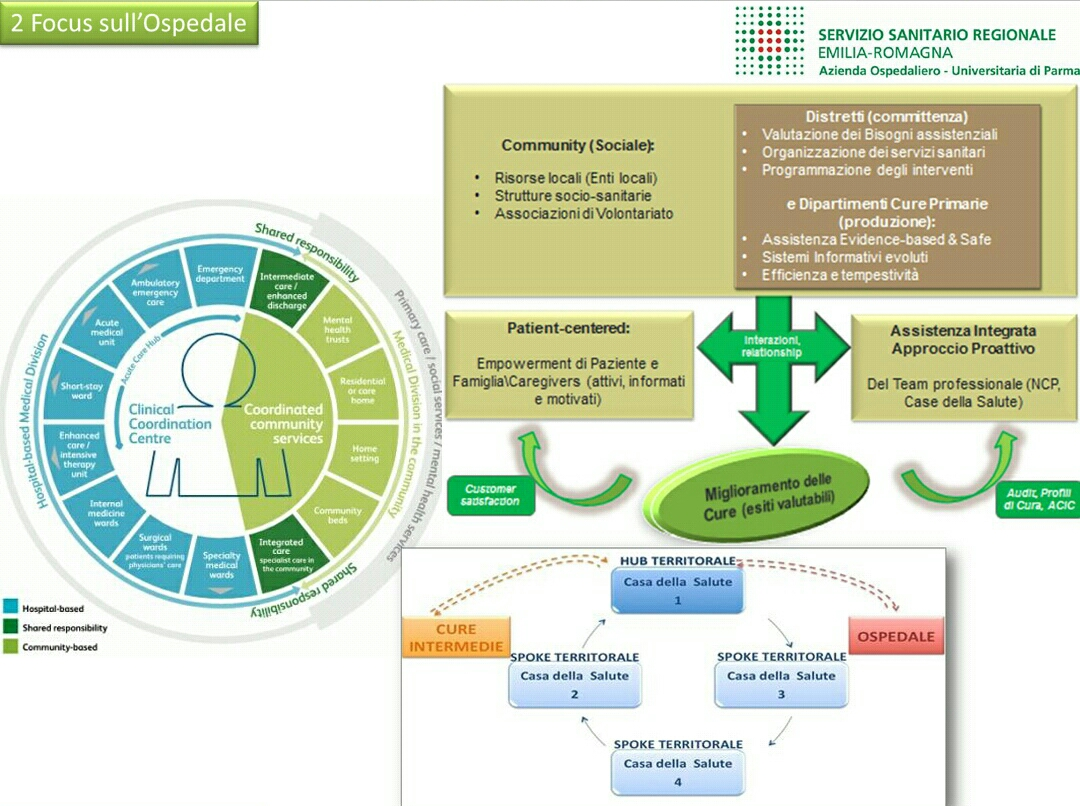
\includegraphics[width=0.8\textwidth]{32/image11.jpeg}
	\end{figure}

Gli ospedali sono snodi delle reti e attori di integrazione.
Introduciamo un altro concetto che è quello degli snodi e delle reti.
All'interno di un'organizzazione esiste un sistema di soggetti, ognuno
dei quali esercita una propria competenza, non gli si chiede di fare
oltre, ma quella competenza la deve garantire. Questo sistema di valori
serve a costruire le reti. La \textbf{rete} è il concetto principe che
oggi anima il modo di fare in sanità e di costruire percorsi
diagnostico-terapeutici. Il concetto della rete, da un punto di vista di
architettura, si fonda proprio su chi fa l'\textbf{hub} per quel
determinato percorso di patologia (nel momento in cui il paziente entra
nel percorso) e su coloro che sono gli \textbf{spoke}: il cerchio e i
raggi. Essere spoke non vuol dire essere ad un livello inferiore, anzi.
Si ha una responsabilità anche maggiore! Se si è nell'hub si ha infatti
tutto l'articolato di questo mondo a disposizione (comprese le
competenze professionali accessorie correlate come può essere un gruppo
di colleghi) mentre se si è spoke molto spesso si è soli nel proprio
ambulatorio di primo livello, probabilmente con la propria
apparecchiatura, e ciò vuol dire avere una competenza tale da saper
presagire e meglio diagnosticare e certificare quel grado di patologia
tale da poter continuare a essere gestita a livello di spoke e non
salire al livello successivo, cosa che a volte succede, l'importante è
che succeda in maniera appropriata. Quando succede in maniera
inappropriata allora ci si interroga sul livello etico della scelta (ti
sei liberato del paziente? Hai preferito una strada diversa forse anche
peccando per situazioni che configgono con l'etica? Negligenza,
imperizia, imprudenza, strafottenza?) Allora no, allora così non
funziona più. Un sistema di regole che vengono violate diventa un
sistema etico che si potrebbe anche rivoltare nei confronti di un altro
sistema organizzativo. Quello diventa uno dei problemi più critici per
chi fa organizzazione, quello di mettere i tasselli a posto, che molto
spesso sono relazionali e comportamentali tra uomini.

Nel momento in cui ho l'ospedale che è il famoso hub a tutti gli effetti
(soprattutto se è un'azienda ospedaliera universitaria) esso si correla
con un mondo della territorialità che è fatta di costituenti (case della
salute in cui ci sono i medici di medicina generale, nuclei di cure
primarie, specialisti ambulatoriali territoriali) che possono governare
secondo un criterio di rotazione determinati quadri di patologia.
Bisogna saper gestire il paziente in modo tale che sia lui ad andare in
una di queste Casa della Salute (la quale ha una funzione di hub
rispetto alle altre) o verso l'ospedale o addirittura verso le cure
intermedie, che sono un'altra modalità di assistenza organizzativa in
cui il paziente con determinati livelli di complessità clinica (e molto
spesso anche socio sanitaria) viene preso in carico dal proprio medico
di medicina generale e dal proprio ambiente di assistenza sanitaria
primaria. Questa è una visione etica nel costruire un sistema
organizzativo, che non vuol dire: ``beh, andiamo tutti quanti in
ospedale'', come succede solitamente quando a capodanno si fanno i
cenoni e il giorno dopo ci si trova con dei carichi massivi in Pronto
Soccorso, ove troviamo tutte le variabili. Anche quella è una scelta
etica nel momento in cui tra quei due soggetti uno prima dell'altro
viene avviato alle cure, uno prima dell'altro viene avviato al posto
letto, uno prima dell'altro viene trattato.

La nuova frontiera dell'etica organizzativa sicuramente nasce da quella
che dovrà essere una sempre maggiore chiarezza e trasparenza di accordo
tra decisori politici e portatori di interesse. Vi introduco tre
concetti che animeranno sempre più il futuro: \textbf{Empowerment},
\textbf{Knowledge}, \textbf{Assessment}.

 \begin{figure}[!ht]
\centering
	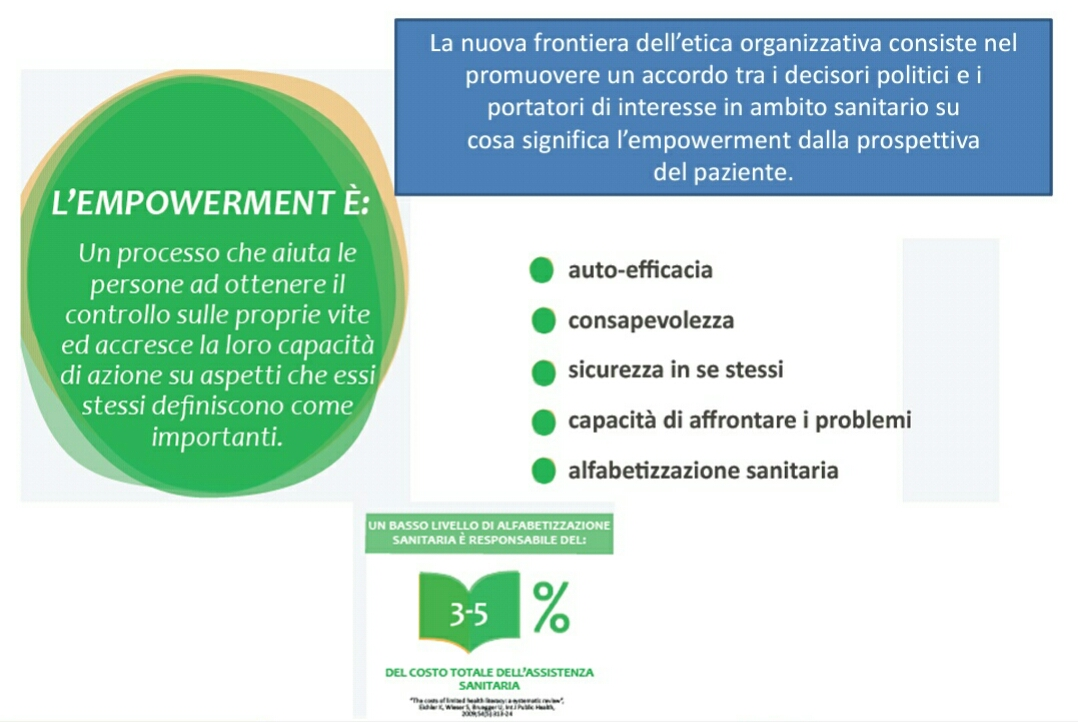
\includegraphics[width=0.8\textwidth]{32/image12.jpeg}
	\end{figure}
	
Empowerment come processo che aiuta le persone ad ottenere il controllo
sulle proprie vite e ad accrescere la loro capacità d'azione su aspetti
che essi stessi definiscono come importanti. Avrete sempre più a che
fare con soggetti che reclamano il proprio empowerment, quindi c'è
bisogno di maggiore consapevolezza del proprio vivere professionale, di
una maggiore capacità nell'affrontare i pazienti, i problemi e di
produrre un'alfabetizzazione sanitaria. Oggi viene calcolato che il 3/5
\% dei costi totali dell'assistenza sanitaria dipendono da un basso
grado di alfabetizzazione.

Ecco le cinque E (poi ne aggiungeremo una sesta) i cinque livelli
applicativi dell'Empowerment che contribuiscono alla sostenibilità del
sistema sanitario:

\begin{itemize}
\item[1.]
  Eguaglianza
\item[2.]
  Esperienza
\item[3.]
  Expertise
\item[4.]
  Engagement
\item[5.]
  Education
\end{itemize}

 \begin{figure}[!ht]
\centering
	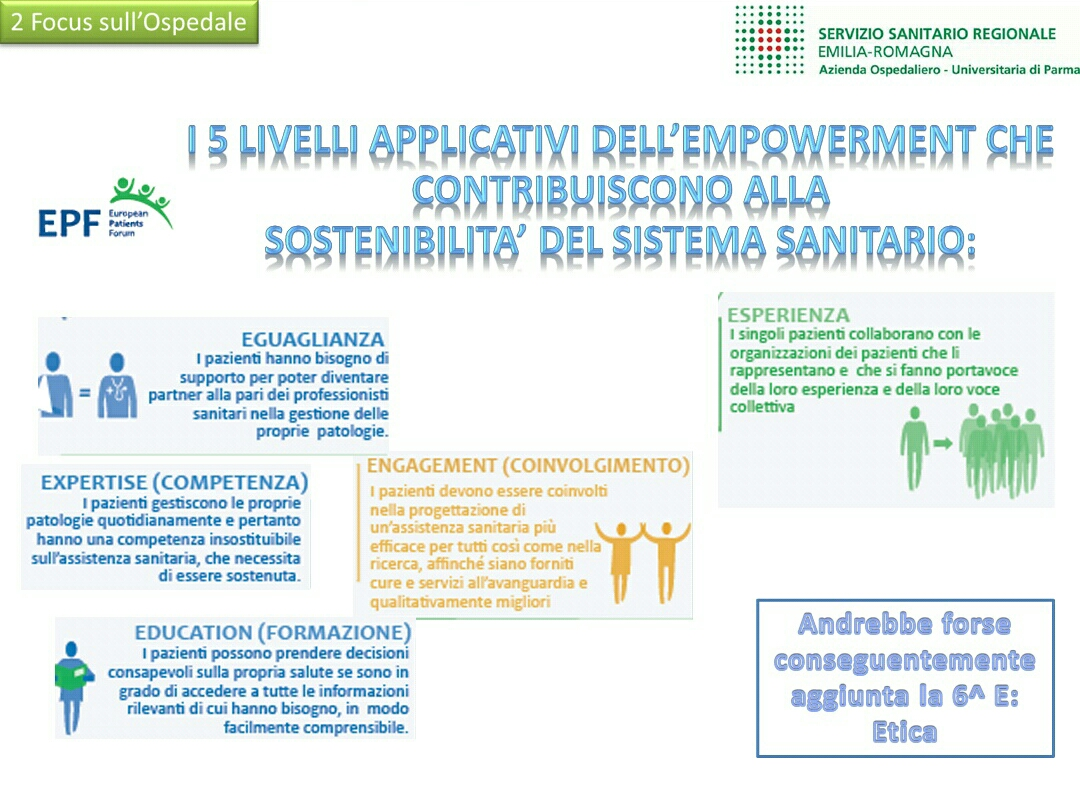
\includegraphics[width=0.8\textwidth]{32/image13.jpeg}
	\end{figure}

Ognuno di questi ha un suo peso ideale, una sua capacità di essere
introiettato nella sfera personale di ciascuno. Queste cinque E
costituiscono gli elementi nodali di una organizzazione che si vuole
eleggere e vuole affermarsi e vuole costruire. A queste cinque E ne
andrebbe aggiunta una, che è quella che permea un poco tutto l'insieme,
che è la E di etica. Noi siamo gestori e quindi ci troviamo a
confrontarci con quelle che sono le dimensioni giornaliere che fanno
parte delle correttezza della persona umana e del professionista.

\subsection{Responsabilità e trasparenza}

Ci sono normative che impegnano chi fa gestione, chi fa managerialità,
chi vive la dimensione professionale. Il Decreto Legislativo 33 del 2013
ha radicato a livello nazionale il concetto della trasparenza e
dell'anticorruzione: è un concetto chiave della pubblica
amministrazione. Se si chiede una macchina, se si chiede un accessorio,
se si pensa ad una innovazione non si può prescindere dal dover
confrontare quella richiesta col panorama esistente, non tanto per
trovare quello al minor costo (anche esso concetto etico che va
affrontato) quanto piuttosto per trovare quella soluzione che garantisca
il miglior rapporto qualità prezzo, in relazione ai bisogni di salute
della popolazione e delle rispose che vogliamo dare al nostro target di
riferimento. Può darsi che non si sia responsabili della situazione in
cui ci si trova (la direzione mi ha mandato questo farmaco, la direzione
mi ha mandato questa macchina) ma lo si diventa se non si fa nulla per
cambiarla (processo a volte non immediato).

 \begin{figure}[!ht]
\centering
	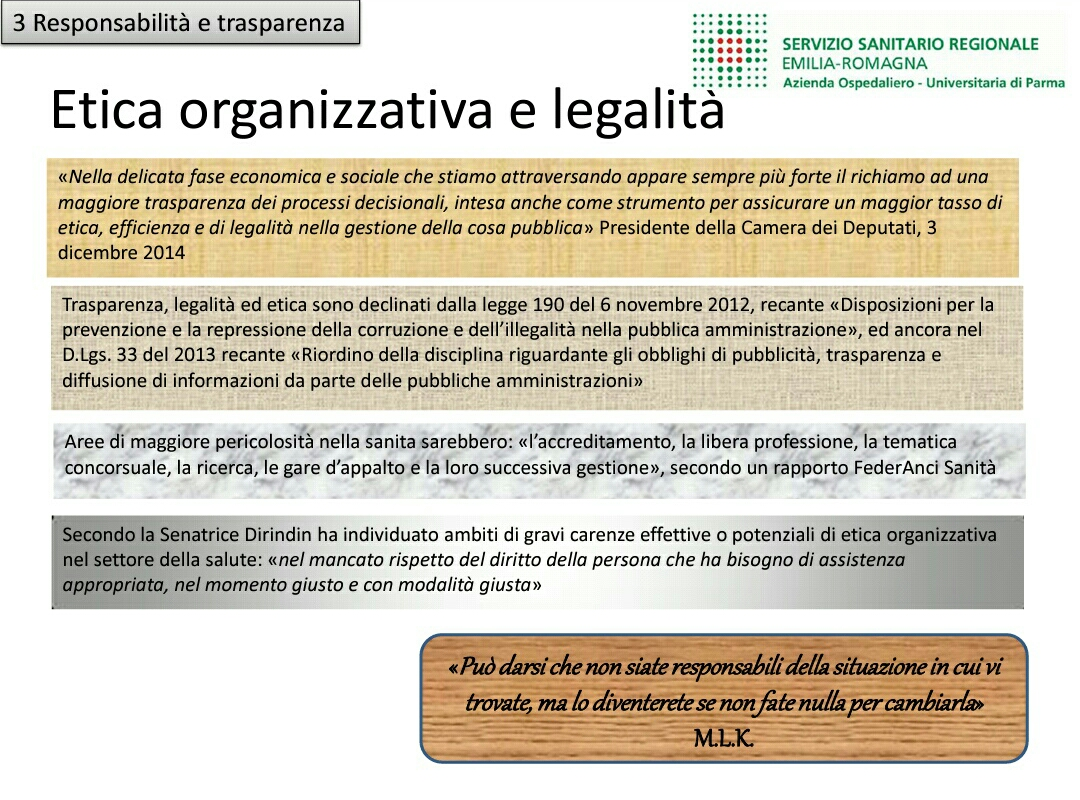
\includegraphics[width=0.8\textwidth]{32/image14.jpeg}
	\end{figure}

La relazione tra etica e violazione della legge, danno economico,
corruzione in senso stretto viene ampiamente descritta e riportata in
letteratura con effetti anche a livello macroeconomico. Si è arrivati
alla trasparenza in sanità soprattutto quando si pensa ai tempi di
attesa: ``devo aspettare 180 gg per avere una RMN, perché quello l'ha
avuto invece in 90 giorni?'' Ecco quindi l'importanza della lista unica,
della lista controllata, anche per le attività operatorie e non solo per
le prestazioni ambulatoriali. Queste situazioni nelle nostre aziende
hanno dei livelli formali di espressione di cui ci rendiamo garanti e
responsabili, perché li andiamo a declinare e li andiamo quindi a
rappresentare.

 \begin{figure}[!ht]
\centering
	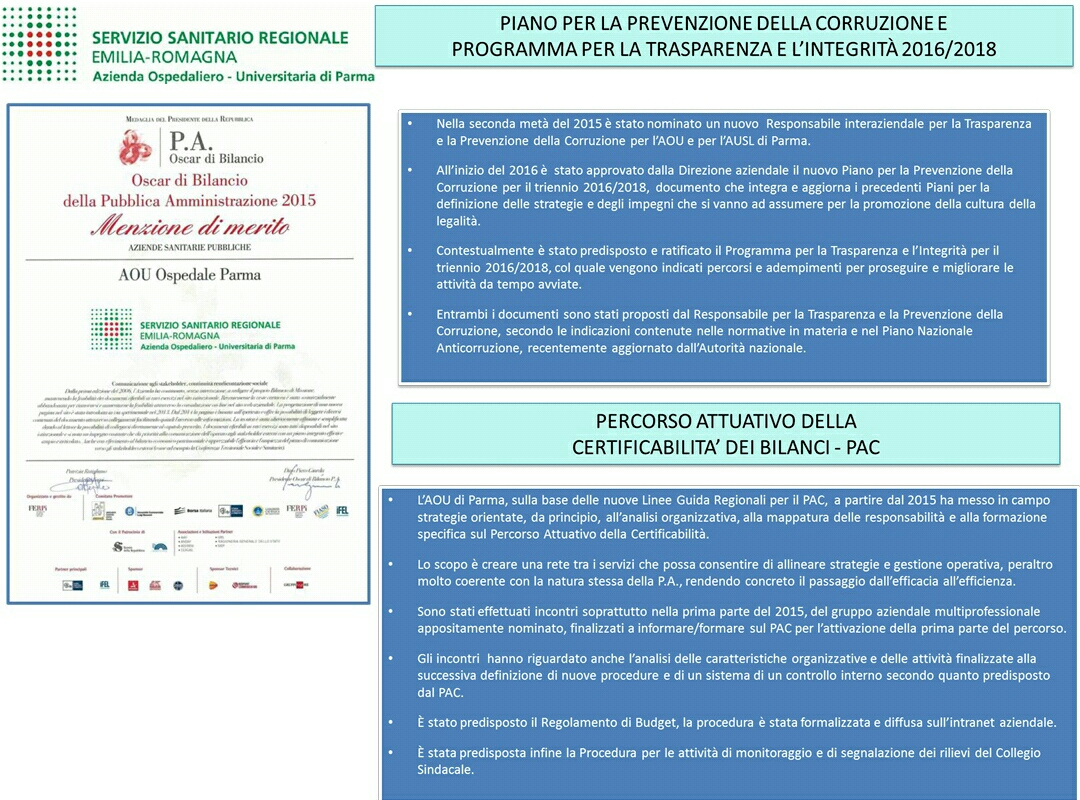
\includegraphics[width=0.8\textwidth]{32/image15.jpeg}
	\end{figure}

Attenzione al concetto di etica nel momento in cui si addentra nel
concetto di responsabilità. Nel momento in cui ci sono delle violazioni
la responsabilità è giuridica (si risponde dei danni) è
politico-amministrativa (riguarda l'equità di accesso ai servizi) è
etica (quando si tratta di spiegare o meno dei comportamenti di buona o
cattiva medicina).

 \begin{figure}[!ht]
\centering
	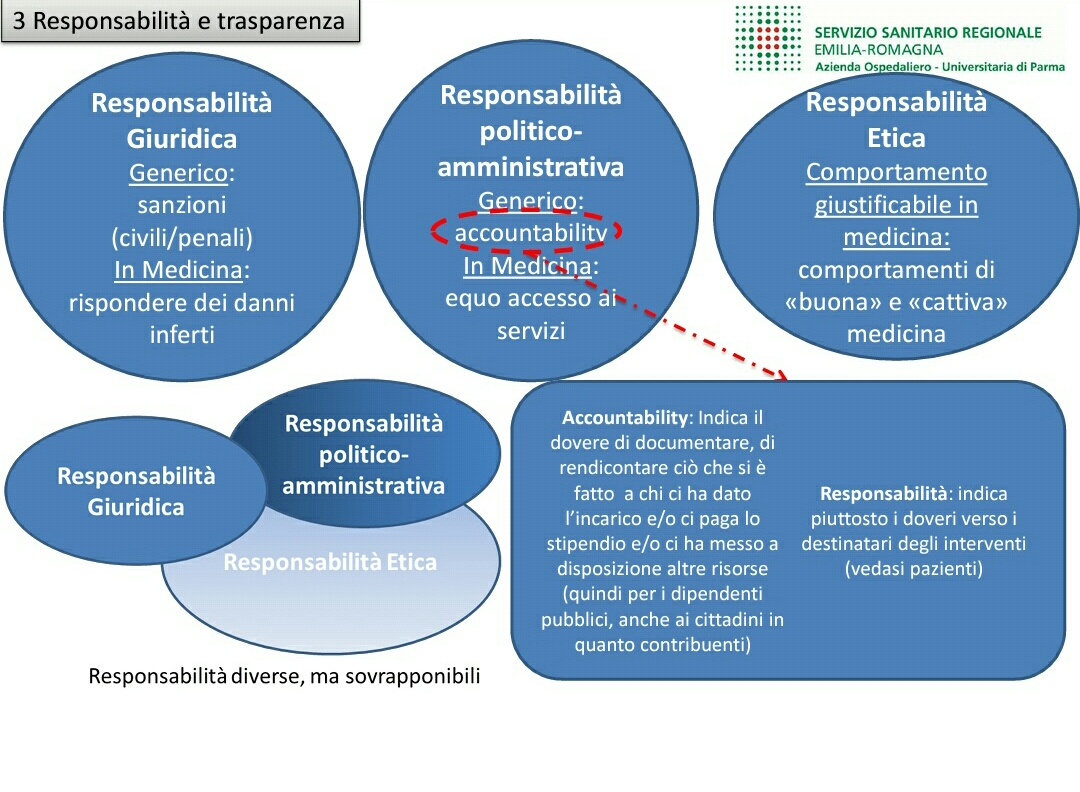
\includegraphics[width=0.8\textwidth]{32/image16.jpeg}
	\end{figure}

Vi volevo introdurre questo concetto: \textbf{accountability}:
l'importanza di documentare, di rendicontare ciò che si è fatto a chi ci
ha dato l'incarico, a chi ci da lo stipendio e ci ha messo a
disposizione altre risorse. C'è la rintracciabilità delle proprie
azioni. Non è solo un concetto di etica, è anche un concetto di
auto-tutela.

 \begin{figure}[!ht]
\centering
	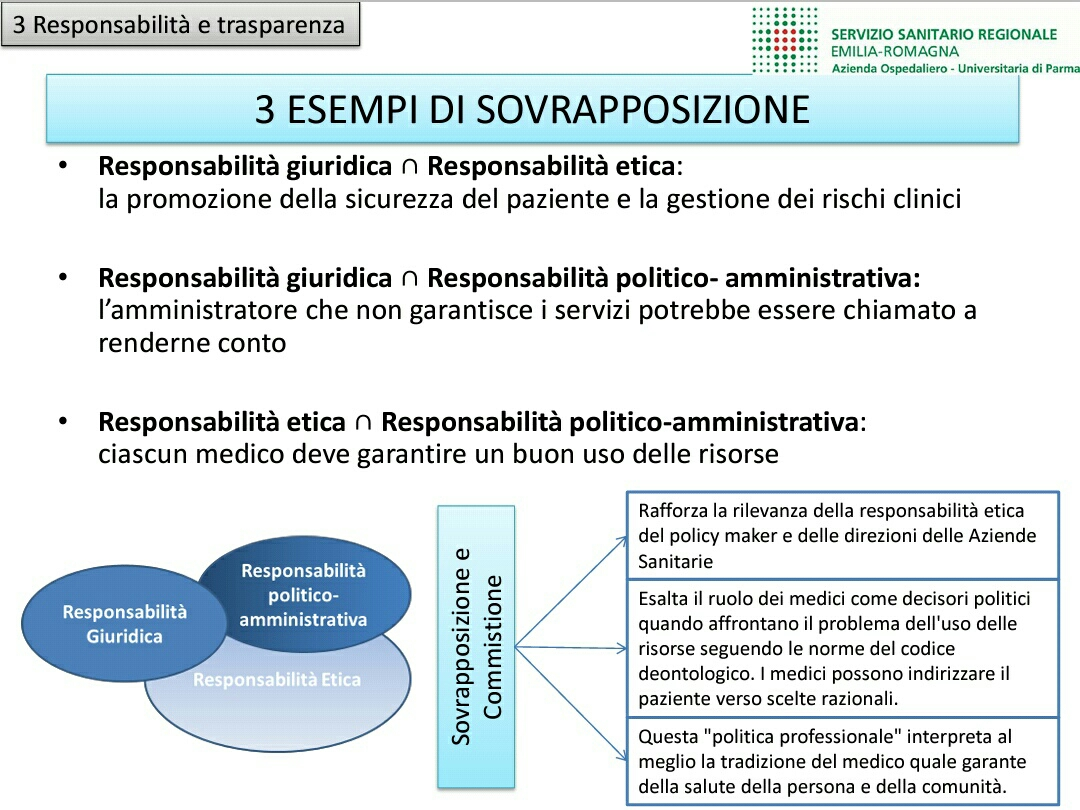
\includegraphics[width=0.8\textwidth]{32/image17.jpeg}
	\end{figure}

C'è un'intersecazione di responsabilità; la responsabilità giuridica
della promozione della sicurezza del paziente e la gestione dei rischi
clinici poi diventa una responsabilità etica. La responsabilità
giuridica dell'amministratore che non garantisce i servizi diventa una
responsabilità politico-amministrativa, ma poi è anche una
responsabilità etica perché ciascun medico deve garantire il buon uso
delle risorse. È un'intersecazione di argomenti, una sovrapposizione,
una commistione, che serve a rafforzare la responsabilità etica di
ciascun medico in quanto decisore. Nel profilo professionale la sfera
deontologica diventa quindi sostanziale.

\subsection{Ruolo della direzione sanitaria e del medico di direzione}

 \begin{figure}[!ht]
\centering
	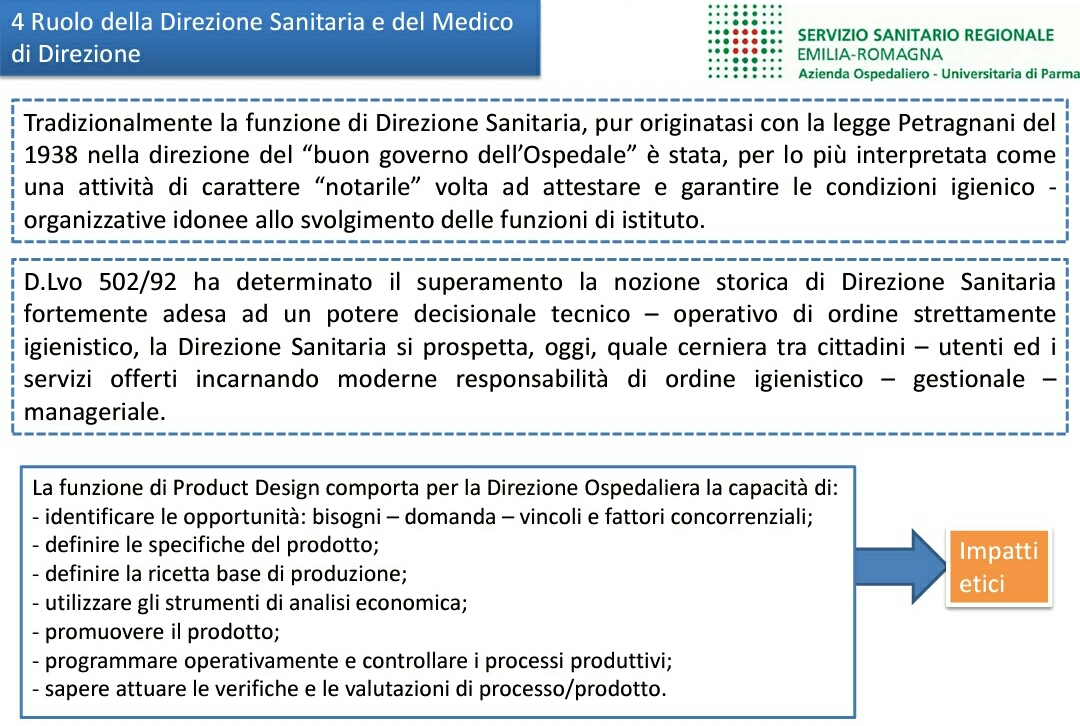
\includegraphics[width=0.8\textwidth]{32/image18.jpeg}
	\end{figure}

Chi di voi sarà un medico di direzione (o si dovrà interfacciare con un
medico di direzione) sappia che sarà in una situazione molto
particolare. Se partiamo dalla legge Petragnani del 1938, il medico di
direzione era il responsabile del buon governo dell'ospedale e una volta
faceva il notaio; oggi ha cambiato molto della sua impostazione, ma
diventa sempre il garante dal punto di vista igienistico, gestionale,
manageriale della tenuta dell'ospedale.

Vi lascio un concetto: un medico (non solamente di direzione) non può
pensare di essere medico se non pensa innanzitutto di essere una
cerniera (non solo quindi ad affrontare in maniera molto spesso dura e
anonima il caso). Si è una cerniera all'interno dell'organizzazione, si
è una cerniera all'interno della famiglia, si è una cerniera con il
proprio paziente nel momento in cui lo si rende consapevole del proprio
stato. Si è cerniere. Se si digerisce questo concetto probabilmente si
interpreterà meglio il proprio ruolo di medici nell'accezione più ampia
e più vasta possibile, a prescindere dalle funzioni specialistiche che
ognuno di voi sarà chiamato a svolgere.

 \begin{figure}[!ht]
\centering
	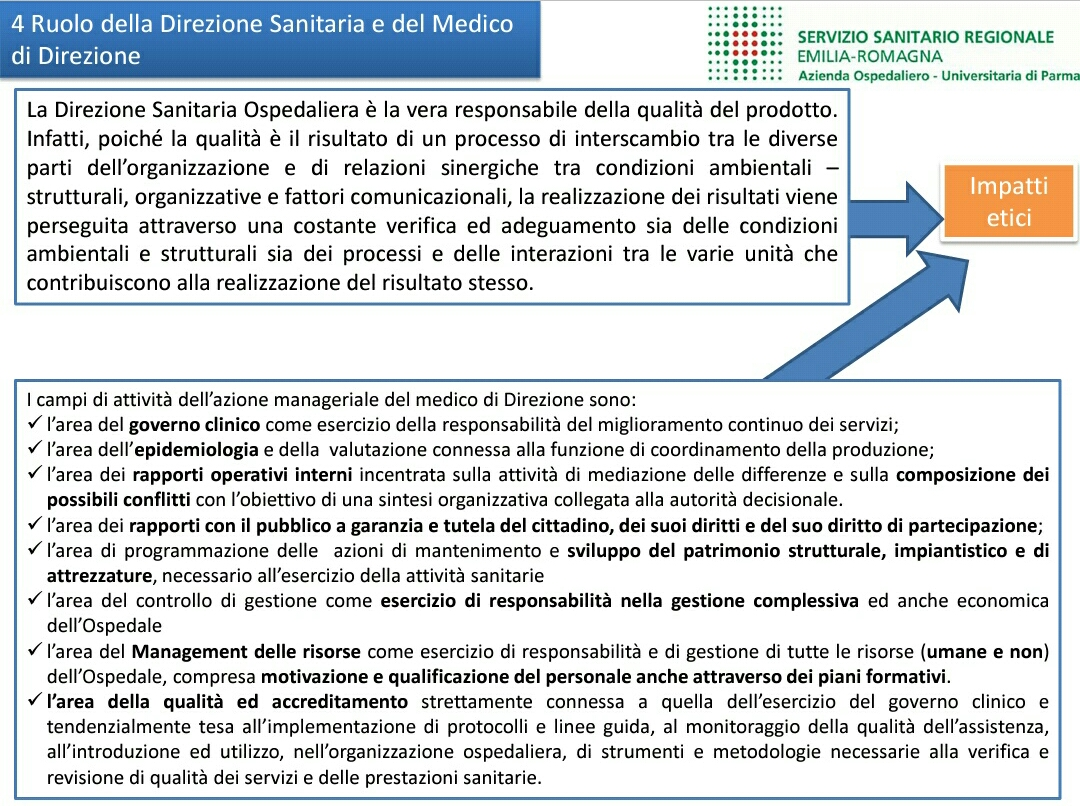
\includegraphics[width=0.8\textwidth]{32/image19.jpeg}
	\end{figure}

\subsection{Formazione e aggiornamento}

Un altro concetto che fa parte del medico, e di come egli interpreta
l'etica, è questo: se il medico pensa alla propria formazione come una
raccolta punti della Coop penso che abbia sbagliato completamente le
proprie scelte di vita. Non è solamente un discorso di quantificazione
di ECM, è un discorso di valorizzazione del capitale umano, che impegna
un'organizzazione perché noi spingiamo i nostri professionisti verso
determinati orientamenti anche formativi; è un discorso di investimenti,
soprattutto perché il costo del lavoro costituisce circa il 50\% dei
costi complessivi di un'azienda. Se non si agisce su questo 50\%
attraverso qualcosa di intangibile che è la formazione (che poi diventa
la cosa più tangibile nel proprio risultato pratico) quel 51\% scritto
nei bilanci rischia di essere anche il 60, il 70, l'80\% come effetti
negativi.

 \begin{figure}[!ht]
\centering
	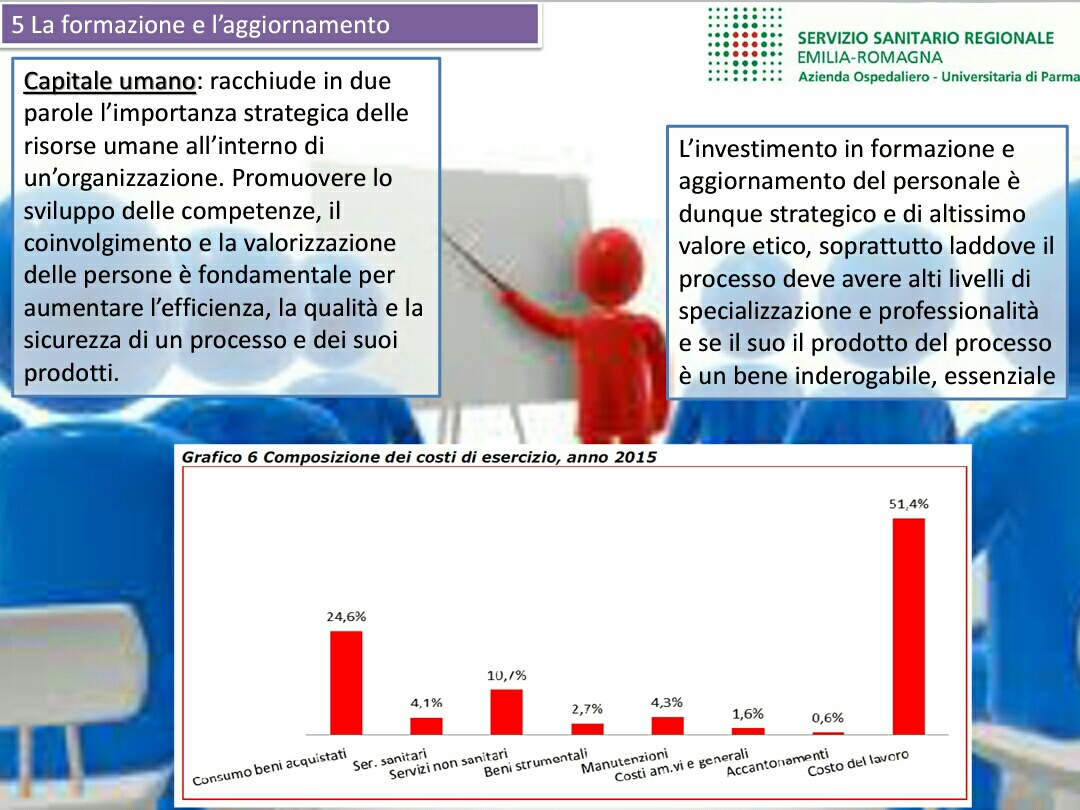
\includegraphics[width=0.8\textwidth]{32/image20.jpeg}
	\end{figure}

Quindi spingere verso l'organizzazione e la formazione vuol dire mettere
insieme i tre assi che costituiscono le matrici di un'organizzazione.

\begin{itemize}
\item[1.]
  L'efficienza della gestione operativa (\textbf{assett}):
  l'organizzazione deve rispondere ai bisogni reali della popolazione di
  riferimento.
\item[2.]
  \textbf{Knowledge}: la specializzazione e la gestione delle competenze
  professionali, il modo in cui noi apparteniamo alle reti strutturate,
  che sono la rete ambientale del nostro reparto, della nostra unità
  operativa, della nostra azienda, del nostro sistema sociale di
  riferimento provinciale nel momento in cui ci interfacciamo con la
  sanità del territorio se siamo ospedalieri, o ospedaliera se siamo dei
  medici territoriali.
\item[3.]
  Il \textbf{disease management}, cioè l'appropriatezza dei percorsi di
  cura. Quello che sto facendo, la mia scelta, è una scelta appropriata?
  Non dimenticate mai un secondo della vostra vita professionale di
  porvi questa domanda. Soprattutto quando vi trovate a ragionare con
  delle vite umane.
\end{itemize}

 \begin{figure}[!ht]
\centering
	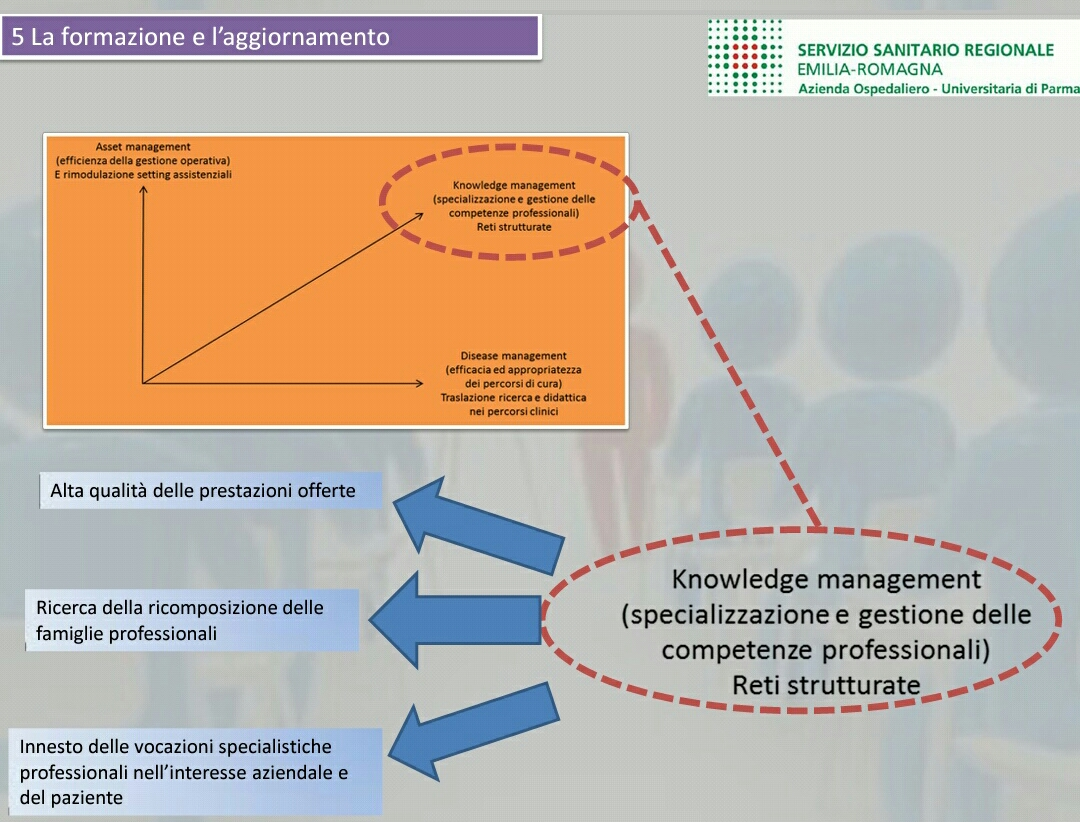
\includegraphics[width=0.8\textwidth]{32/image21.jpeg}
	\end{figure}

\subsection{Ruolo dei comitati etici in aziende ospedaliero-universitarie}

In ospedale, come nelle aziende sanitarie, esiste il comitato etico, un
organismo indipendente che governa determinate scelte che vengono fatte
da gruppi professionali nel momento in cui questi scelgono di portare
avanti delle sperimentazioni; è un organismo terzo che garantisce la
tutela della salute (ovvero che quelle sperimentazioni avvengano secondo
criteri di coerenza a normative di carattere internazionale, come la
Carta dei diritti dell'Uomo).

 \begin{figure}[!ht]
\centering
	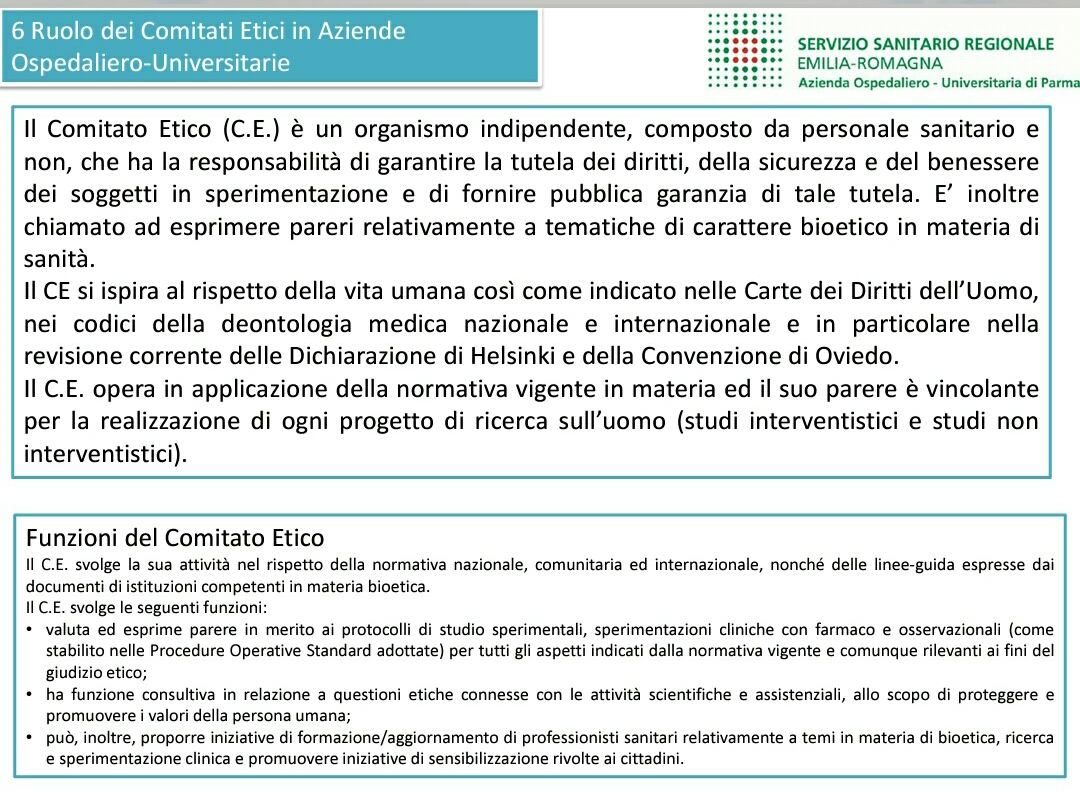
\includegraphics[width=0.8\textwidth]{32/image22.jpeg}
	\end{figure}

\subsection{Esempi pratici di progetti di riorganizzazione sanitaria in AzOU e impatti etici}

Quando si fa etica in un'organizzazione poi bisogna anche leggere che
cosa abbiamo realizzato e che cosa stiamo realizzando. Se un'azienda
decide di realizzare un Polo Oncologico, molto complesso, questa è una
scelta di responsabilità enorme, è una scelta sociale, in cui la valenza
etica è fondamentale. Se un'azienda decide di applicare il progetto
SIGLA (Sistema Integrato Gestione Liste d'Attesa, cioè la correttezza
con cui i medici devono mettere i propri pazienti in lista di attesa,
sia per l'ambulatoriale che per le attività operatorie) c'è una valenza
etica a monte di tutto ciò. Se si avviano dei progetti sulla fragilità
lo si fa per difesa della persona umana, per inserirla all'interno di
percorsi che siano il più possibile funzionali a quel bisogno. E cosi
dicasi per i percorsi diagnostico-terapeutici e per tutte quelle
innovazioni che abbiamo cercato brevemente in questa rassegna di
descrivervi.

 \begin{figure}[!ht]
\centering
	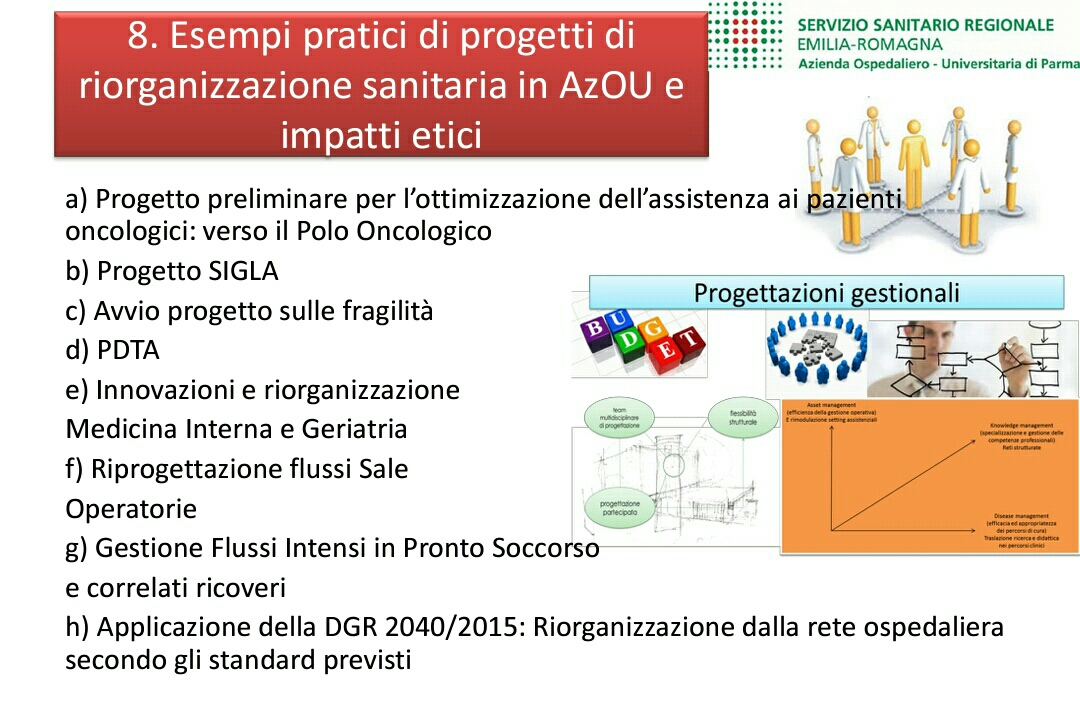
\includegraphics[width=0.8\textwidth]{32/image23.jpeg}
	\end{figure}

C'è una corrispondenza, un carattere univoco di relazione tra scelte
organizzative e applicazioni di criteri che sono quelli su cui si basa
da sempre il vivere sociale o su cui si sono articolate le motivazioni e
i principi fino ad ora elencati, che fanno parte dello sviluppo del
profilo del medico, non solo di quello che fa organizzazione ma di
qualsiasi figura professionale. I discorsi sulla continuità
assistenziale, sull'interdisciplinarità e sul rispetto dell'assistito
fanno parte di scelte che hanno a monte dati epidemiologici che possono
essere letti in doppio: com'era prima e com'è dopo aver fatto un
intervento organizzativo. Questo è fondamentale, sapere sempre da dove
si parte, dove si arriva e soprattutto avere sempre una proiezione di un
futuro anche molto lontano dal nostro.

 \begin{figure}[!ht]
\centering
	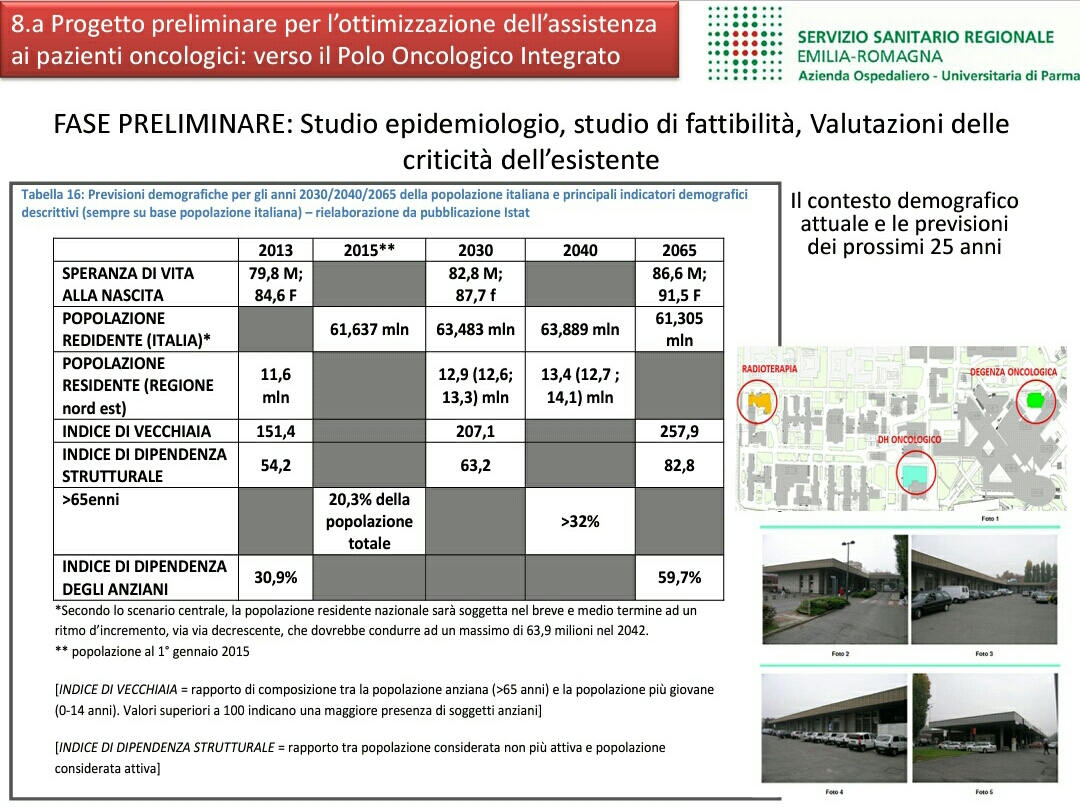
\includegraphics[width=0.8\textwidth]{32/image24.jpeg}
	\end{figure}

Quando noi parliamo del polo oncologico, abbiamo fatto uno studio su
come cambia la speranza di vita e sui bisogni della popolazione di
Parma, ma non dal 2013 al 2015, ci siamo proiettati al 2065!

Quando si lavora, si lavora per mettere dei valori aggiunti nel proprio
sistema; quando lo si lascia, lo si lascia vedendo il valore aggiunto
frutto del proprio passaggio, perché poi si passa un testimone. E questo
è sostanziale nel modo di essere etici nel gestire l'organizzazione. Un
esempio di scelta è quello di variare l'orario di ingresso del
day-hospital e vedere che la gente non sta al freddo dalle 7 alle 8, ma
la mattina alle 7 entra nel day-hospital oncologico. Questo è un esempio
dell'agire dell'organizzazione e del creare dei presupposti per il
cambiamento.

 \begin{figure}[!ht]
\centering
	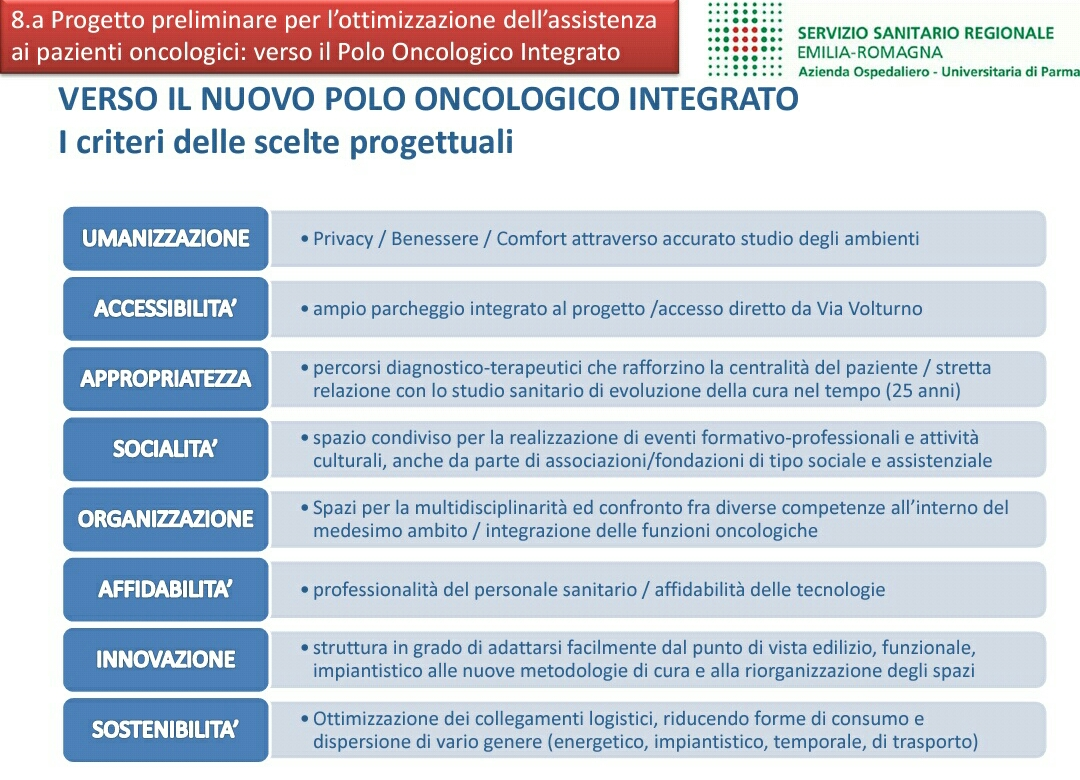
\includegraphics[width=0.8\textwidth]{32/image25.jpeg}
	\end{figure}

Queste sono immagini del futuro che verrà. Bisogna essere un po'
visionari se si vuole essere eticamente coerenti, perché a volte bisogna
spingere il cuore oltre lo steccato. Questo è quello che verrà a Parma
in termini di Polo Oncologico Integrato, che si interfaccerà con la
Torre delle Medicine, diventando un centro dedicato per i pazienti
oncologici dove verranno svolte attività non solo di terapia, ma anche
di diagnostica e di radioterapia.

Questo è invece un progetto di riorganizzazione di sale operatorie,
costruito con almeno 80 colleghi, tra chirurghi e medici di varie
specialità.

Gestire i flussi di pronto soccorso non è solamente un criterio di
carattere giornalistico, ma segue delle regole di tecnica per cui i
flussi vengono monitorati giornalmente (i flussi di popolazione rispetto
alla disponibilità di posti letto); vengono monitorati e interpretati
rispetto a quelli che sono gli strumenti della tecnica epidemiologica
soprattutto quando sono flussi di carattere stagionale. Quantificare dal
punto di vista statistico i fenomeni è uno degli strumenti per poter
gestire l'organizzazione e quindi avere gli elementi opportuni per poi
fare le scelte.

 \begin{figure}[!ht]
\centering
	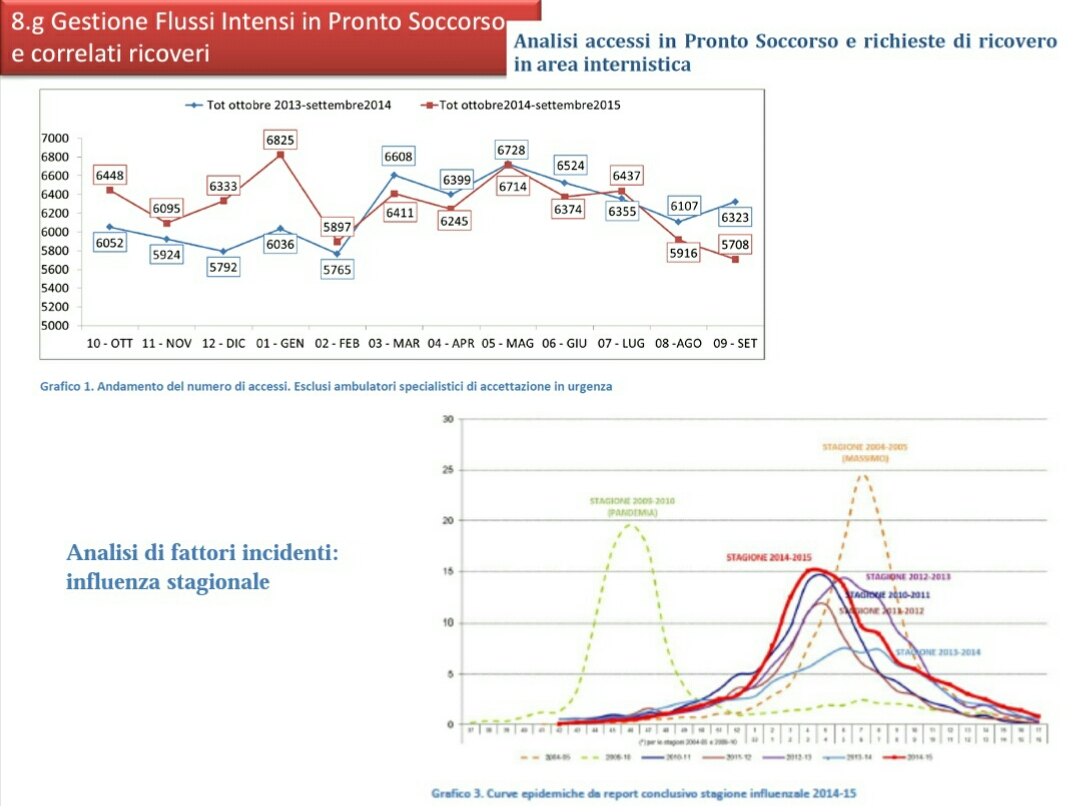
\includegraphics[width=0.8\textwidth]{32/image26.jpeg}
	\end{figure}

\subsection{Conclusioni del Dottor Balestrino}

A partire dai codici etici e deontologici e attraverso lo strumento
organizzativo ed istituzionale del Comitato Etico, l'importante è che si
sviluppi una cultura che integri a tutti i livelli i processi
decisionali. Sicuramente chi riveste un ruolo di leadership in
un'azienda ha una responsabilità, quindi mai tenere disgiunto il
concetto della valenza etica dal concetto di responsabilità. Esiste una
relazione tra organizzazione sanitaria e società e tale relazione si
esplicita ricorrendo al concetto di mandato fiduciario. Quando il
direttore generale dice che i nostri pazienti sono i nostri datori di
lavoro, non è che dice una cosa di poco conto. Non facciamo un piacere
ad alcuno a lavorare nella struttura e nella struttura pubblica. Semmai
è l'inverso. Se siamo meritevoli di quel mandato fiduciario la gente
viene, sa parlare di noi e ci mette in condizione di essere quello che
siamo. La relazione del bisogno sanitario non è univoca e
monodirezionale, questo deve permeare la coscienza di molti. Esiste a
monte ancora una capacità di scelta e soprattutto una valenza
nell'esprimersi e anche a volte nel reclamare, che noi viviamo quando
lavoriamo onestamente. A volte quando troviamo qualcuno che si lamenta
diciamo ``e caspita, oltre l'anima non si può dare''. Però chissà, ci si
interroga sempre se quel nostro essere in un ambiente trova quel nostro
impegno corrispondente al nostro vicino professionale che lo esplicita
nella stessa maniera e valenza con cui lo esprimiamo noi. È etico, nel
caso, richiamare quel nostro collega a quei valori e a quegli obiettivi
che io cerco di perseguire? Ha senso quindi quell'espressione di
disapprovazione o di disaffezione? L'organizzazione sanitaria riceve
dalla società un mandato, quello di soddisfare i bisogni di salute, da
qui il concetto di ruolo sociale dell'agire medico. Il modo in cui la
gente soffre e muore è un modo sociale, pertanto la struttura delle cure
della salute è inseparabile dall'organizzazione generale della società.
Nel momento in cui facciamo salute, all'interno di ambienti destinati a
fare salute, noi siamo un pezzo della società cui apparteniamo, agiamo
con delle competenze per eseguire un compito. Ma siamo sempre un pezzo
di un'espressione sociale e quindi come tale abbiamo maggiormente la
responsabilità di saperla interpretare.

 \begin{figure}[!ht]
\centering
	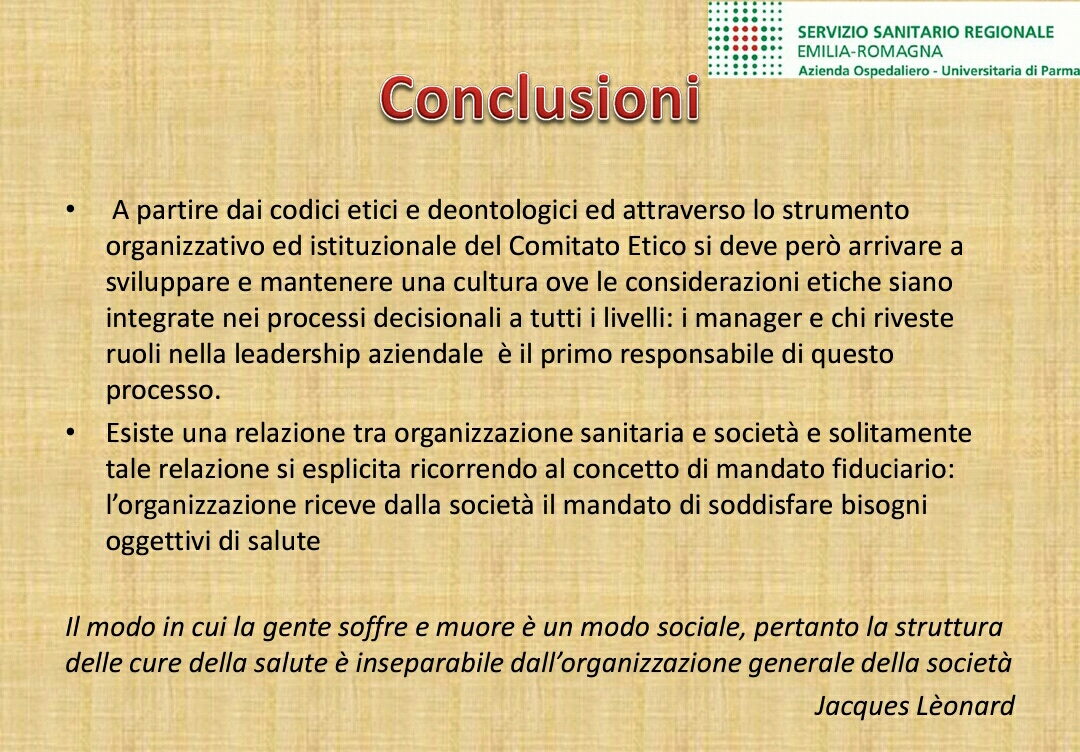
\includegraphics[width=0.8\textwidth]{32/image27.jpeg}
	\end{figure}

\subsection{Conclusioni del Dottor Muzzetto}

Elementi che voi state acquisendo e che in apparenza sembrano inutili,
sono in realtà di grande utilità: la formazione, il rapporto con gli
altri, il lavorare nel sistema sanitario, il lavorare come medici di
famiglia, l'entrare nel sistema delle specializzazioni nella medicina
pubblica e anche nell'ambito universitario. Anche il rischio clinico,
che sembra avulso dalla realtà e anche da un insegnamento di etica,
rientra nel grande capitolo dell'etica. Era bellissimo quel rilievo
fatto sulla morale come principio assoluto e condiviso, difficilmente
modificabile, e sull'etica individuale o collettiva di adattamento alle
novità e ai cambiamenti, ma in maniera tale che quei principi morali non
possano essere in qualche modo deviati, distorti o non considerati. C'è
una collaborazione stretta tra chi è tutore della deontologia e
dell'etica professionale e chi in questo momento sta gestendo un
problema di valutazione della cura e dell'assistenza e lo vede con un
taglio etico. C'è un messaggio importante da dare alle nuove generazioni
di medici e alle vecchie generazioni: non possiamo pensare che le
responsabilità siano di altri! Le responsabilità son sempre nostre,
dobbiamo sempre metterci in discussione e ci si mette in discussione
affrontando i problemi ma anche apprendendo le novità, cioè entrando
nella formazione che non è un creditificio, ma è l'acquisizione di
nozioni importanti.

\subsection{Intervento conclusivo del Dottor Fabi}

Durante il corso di laurea in medicina e chirurgia, ma anche delle
professioni sanitarie, si impara prima di tutto una tecnica (conoscere,
essere informati sugli ultimi aggiornamenti nelle materie e nelle
discipline) ma bisogna uscire con la consapevolezza che c'è un sapere
che deve essere applicato concretamente. Non si lavorerà più da soli: 50
anni fa la medicina poteva anche essere esercitata in solitudine, oggi
sono prevalenti le malattie croniche. Le malattie croniche non possono
essere curate in solitudine, c'è bisogno di una integrazione e
concatenazione di prestazioni che è fatta dal lavoro di equipe; il
lavoro di equipe c'è in ospedale e c'è sul territorio. Non c'è più il
medico condotto sul territorio, non c'è più il grande clinico
ospedaliero che, con l'occhio clinico e la visione derivante dalla
semeiologia fisica tradizionale, fa diagnosi oppure rispedisce a casa
guariti. Non siamo soli adesso, e non lo sarete voi. Il vostro sapere
disciplinare applicato, quindi il vostro saper fare, non può prescindere
dai contesti organizzativi. Bisogna conoscere quei contesti
organizzativi, bisogna essere in grado di lavorare in equipe e in
squadra. Chi non è capace, come medico e come professionista, di
lavorare in equipe si esclude da un percorso di cura di alto livello
qualitativo. Non è più sufficiente la capacità, il sapere o la nozione,
perché molte volte ci sono pazienti che, come nozioni, ne sanno molto
più dei medici. Molte volte la nozione che il paziente apprende dai
mezzi di comunicazione o da internet, senza una mediazione, è solo
nozione, non diventa cultura. Avrete sempre più a che fare con dei
pazienti, malati cronici, che decideranno loro qual è il livello di
salute che ritengono compatibile con il proprio benessere percepito.
Gran parte della popolazione mondiale vive ancora lottando contro le
malattie acute, mentre noi viviamo in un mondo fortunato e privilegiato,
ove l'aspettativa di vita è doppia o tripla rispetto al resto del mondo.
Ad un malato di polmonite bisogna dare un antibiotico e anche qua entra
in gioco l'etica: l'antibiotico deve essere quello efficace e
appropriato, quello necessario e anche quello più economico perché se
noi investiamo risorse eccessive e non utili per curare quella
situazione, le sottraiamo a qualcun altro che ne ha necessità. Ecco
l'eticità professionale delle scelte. Abbiamo a che fare non solo con la
malattia acuta ma prevalentemente con quella cronica. Chi ha una
malattia neurologico-degenerativa e arriva nella fase di progressione
della stessa, deve scegliere, insieme all'equipe che lo cura, se
utilizzare mezzi meccanici per sostenere la capacità respiratoria, se
usufruire della nutrizione artificiale per mantenersi idratato e
nutrito. In questi casi troviamo gente che sceglie di non farlo. Anche
se, considerando l'organismo come macchina (e il modello biomedico lo
considera tale) il dovere del medico è quello di prescrivere in quel
caso il supporto ventilatorio e la nutrizione artificiale. Dovremo far
sì che il paziente riesca ad avere l'informazione e gli strumenti per
applicare quell'informazione (empowerment); non ci si deve limitare ad
una delega (``ora sono fatti tuoi, io ti ho dato le informazioni, ora
arrangiati''), ma bisogna aiutare e supportare il paziente nella scelta.
I valori dell'integrazione, della cooperazione professionale,
dell'interdipendenza (le scelte che facciamo sono sempre negoziate con i
colleghi all'interno dell'equipe quando curiamo un paziente con una
patologia cronica), della reciprocità nella relazione tra i
professionisti \ldots{} sono tutti valori alla base del comportamento
professionale.

La riorganizzazione delle chirurgie è un progetto in corso: stiamo
riorganizzando le aree chirurgiche in modo che le liste di attesa dei
pazienti che devono accedere all'intervento vengano definite non per
singolo medico che ha in carico il paziente (e che ha quella sala
operatoria che considera come una proprietà individuale, o i posti letto
che considera come suoi); le risorse (sala operatoria, posto letto,
ambulatorio ecc) verrebbero quindi scelte e definite in un percorso di
negoziazione tra i professionisti in relazione alle priorità cliniche
che hanno i pazienti (priorità cliniche cronologiche).

La fatica che si sta facendo in questo momento è notevole. Si sta
cercando di far apprendere ai professionisti (noi compresi che siamo
stati formati 30 anni fa, quando il modello della malattia era
completamente diverse) modalità di lavoro nuove, come ad esempio il
lavoro in equipe. Voi siete nella fase di crescita professionale e anche
personale in cui state formando le vostre attitudini al lavoro di
equipe, e questa non è nozione, queste sono le norme e i valori che
ispirano i comportamenti. Più cercate di contribuire a questi
cambiamenti una volta entrati nella professione tanto più portate
dell'arricchimento del capitale intellettuale (di cui voi siete i
portatori) che sarà l'innovazione della sanità del futuro, sia negli
ospedali sia sul territorio. Ci sono scelte alternative? Non ce ne sono.
Se non altro perché ce lo dice l'epidemiologia, ce lo dice la
demografia.

La salute è un diritto dell'individuo ed un interesse della collettività
(articolo 32 della Costituzione), questo diritto viene garantito
attraverso i LEA (altra scelta etica, poiché lo Sato dice ``queste
prestazioni ve le do perché tutelano quel diritto, queste prestazioni
invece non ve le do perché non hanno evidenza di efficacia'') e resi
compatibili con le risorse messe a disposizione. Noi abbiamo un SSN
finanziato con la fiscalità generale; ogni cittadino che dovrebbe pagare
le tasse in proporzione alle attività svolte e al proprio reddito
contribuisce a finanziare un sistema che è garanzia per sé stesso e per
gli altri (diritto dell'individuo ed interesse della collettività); è
per questo che i cittadini sono i nostri datori di lavoro.